\documentclass[10pt]{IEEEtran}
\usepackage{etex}
%\usepackage{empheq}
\usepackage{epsfig}
\usepackage{amsmath}
\usepackage{multirow}
\usepackage{tabularx}
\usepackage{booktabs}
\usepackage{amsmath,graphicx}
\usepackage{pgf}
\usepackage{tikz}
\usepackage{subfig}
\usetikzlibrary{backgrounds,shapes,snakes}
\usetikzlibrary{calc,chains,positioning}
\usepackage{phaistos}
\usepackage{cases}
\usepackage{pgfplots}
\usepackage{empheq}
\usepackage{cite}
\usepackage{url}

%\renewcommand{\baselinestretch}{0.9}

\begin{document}

\newlength\figureheight
\newlength\figurewidth
\setlength\figureheight{3.0cm}
\setlength\figurewidth{0.37\textwidth}

% %
\title{Signal-Dependent Penalty Functions for \\ Robust Acoustic Multi-Channel Equalization}

\author{%
  Ina~Kodrasi,~\IEEEmembership{Member,~IEEE} and Simon~Doclo,~\IEEEmembership{Senior Member,~IEEE}
  \thanks{The authors are with the Signal Processing Group, Department of Medical Physics and Acoustics, and Cluster of Excellence Hearing4All, University of Oldenburg, Germany (e-mail: ina.kodrasi@uni-oldenurg.de, simon.doclo@uni-oldenburg.de).}%
  \thanks{
This work was supported in part by the Cluster of Excellence 1077 ``Hearing4All'', funded by the German Research Foundation (DFG), the Marie Curie Initial Training Network DREAMS (Grant no. 316969), and the joint Lower Saxony-Israeli Project ATHENA, funded by the State of Lower Saxony.
}
}
% make the title area
\maketitle
\newpage

\begin{abstract}
\boldmath
Acoustic multi-channel equalization techniques, which aim to achieve dereverberation by reshaping the room impulse responses~(RIRs) between the source and the microphone array, are known to be highly sensitive to RIR perturbations.
In order to increase the robustness against RIR perturbations, several {\emph{signal-independent}} methods have been proposed, which only rely on the available perturbed RIRs and do not incorporate any knowledge about the output signal.
% The multiple-input/output inverse theorem (MINT) technique, which aims to invert the room impusle responses~(RIRs) between the source and the microphone array, is known to be highly sensitive to RIR perturbations. 
% To increase robustness, partial equalization techniques such as relaxed multi-channel least-squares (RMCLS) and partial multi-channel equalization based on MINT (PMINT) have recently been proposed.
% In addition, several signal-independent methods have been proposed to further increase the robustness of the MINT, RMCLS, and PMINT techniques, such as designing approximate filters in the subband domain or incroporating regularization.
This paper presents a novel {\emph{signal-dependent}} method to increase the robustness of equalization techniques by enforcing the output signal to exhibit spectro-temporal characteristics of a clean speech signal. 
Motivated by the sparse nature of clean speech, we propose to extend the cost function of state-of-the-art least-squares equalization techniques, i.e., the multiple-input/output inverse theorem (MINT), relaxed multi-channel least-squares~(RMCLS), and partial multi-channel equalization based on MINT (PMINT), with a signal-dependent penalty function promoting sparsity of the output signal in the short-time Fourier transform domain. 
Three conventionally used sparsity-promoting penalty functions are investigated, i.e., the $l_0$-norm, the $l_1$-norm, and the weighted $l_1$-norm, and the sparsity-promoting reshaping filters are iteratively computed using the alternating direction method of multipliers.
Simulation results for several acoustic systems and RIR perturbations demonstrate that incorporating sparsity-promoting penalty functions significantly increases the robustness of MINT, RMCLS, and PMINT, with the weighted $l_1$-norm typically outperforming the $l_0$-norm and the $l_1$-norm.
Furthermore, it is shown that the weighted $l_1$-norm sparsity-promoting PMINT technique outperforms the other sparsity-promoting techniques in terms of perceptual speech quality.
Finally, it is shown that the signal-dependent weighted $l_1$-norm sparsity-promoting PMINT technique yields a similar or better dereverberation performance than the signal-independent regularized PMINT technique, confirming the advantage of using signal-dependent penalty functions for robust dereverberation filter design.
\end{abstract}
\begin{IEEEkeywords}
acoustic multi-channel equalization, sparsity, signal-dependent penalty function, ADMM
\end{IEEEkeywords}

\section{Introduction}

\IEEEPARstart{I}{N} many hands-free speech communication applications such as teleconferencing, voice-controlled systems, or hearing aids, the recorded microphone signals do not only contain the desired signal, but also attenuated and delayed copies due to reverberation.
Reverberation causes signal degradation, typically leading to decreased speech intelligibility~\cite{Beutelmann_2006,Goetze_AES_2010,Warzybok_IWAENC_2014} and performance deterioration in automatic speech recognition systems~\cite{Yoshioka_ISPM_2012,Xiong_EURASIP_2015}.
Hence, in the last decades several single- and multi-channel dereverberation techniques have been proposed~\cite{Naylor_Derev_book}, with multi-channel techniques being generally preferred since they enable to exploit both the spectro-temporal and the spatial characteristics of the microphone signals. 
Existing multi-channel dereverberation techniques can be broadly classified into: i) spectral enhancement techniques aiming at suppressing the late reverberation in the spectral domain based on an estimate of the late reverberant power spectral density~\cite{Lebart_ACUSTICA_2001,Habets2009a,Braun_EURASIP_2015,Kuklasinski_ITASLP_2016}, ii) probabilistic modeling-based techniques aiming at blindly estimating the parameters of statistical models assumed to represent the clean speech signal and the room impulse responses~(RIRs)~\cite{Nakatani_ITASLP_2010,Schmid_ITASLP_2014,Schwartz_ITASLP_2015,Jukic_ITASLP_2015}, and iii) acoustic  multi-channel equalization techniques aiming at reshaping the available (measured or estimated) RIRs between the source and the microphone array~\cite{Miyoshi_ITASS_1988, Kallinger_ICASSP_2006,Jungmann_ITASLP_2012, Lim_ITASLP_2014, Kodrasi_ITASLP_2013, Rashobh_ITASLP_2014}.
Unlike spectral enhancement and probabilistic modeling-based techniques, acoustic multi-channel equalization techniques can in theory achieve perfect dereverberation~\cite{Miyoshi_ITASS_1988,Hacihabibouglu_ITASLP_2012}, therefore comprising an attractive approach to speech dereverberation.

A well-known multi-channel equalization technique aiming at acoustic system inversion is the multiple-input/output inverse theorem~(MINT) technique~\cite{Miyoshi_ITASS_1988}, which however suffers from drawbacks in practice. 
Since the available RIRs typically differ from the true RIRs due to fluctuations~(e.g., temperature or position variations~\cite{Radlovic_ITSA_2000}) or due to the sensitivity of blind system identification~(BSI) and supervised system identification~(SSI) methods to near-common zeros or interfering noise~\cite{Khong_ICASSP_2008,Haque_SPL_2008,Hu_EUSIPCO_2015}, MINT fails to invert the true RIRs, possibly leading to severe distortions in the output signal~\cite{Hikichi_EURASIP_2007,Kodrasi_ITASLP_2013,Lim_ITASLP_2014}.

In order to increase the robustness against RIR perturbations, partial multi-channel equalization techniques such as relaxed multi-channel least-squares~(RMCLS)~\cite{Lim_ITASLP_2014} and partial multi-channel equalization based on MINT~(PMINT)~\cite{Kodrasi_ITASLP_2013} have been recently proposed. 
Since early reflections tend to improve speech intelligibility~\cite{Arweiler_JASA_2011,Warzybok_JASA_2012} and late reflections are the major cause of speech intelligibility degradation, the objective of these techniques is to suppress only the late reflections.
Although partial equalization techniques can be significantly more robust than MINT, their performance still remains rather susceptible to RIR perturbations~\cite{Kodrasi_ITASLP_2013}.
As a result, several methods have been proposed to further increase the robustness against RIR perturbations.
In~\cite{Gaubitch_ITASLP_2009,Lim_EUSIPCO_2013} it has been proposed to relax the constraints on the filter design by constructing approximate dereverberation filters in the subband domain.
In~\cite{Kodrasi_EUSIPCO_2012} it has been proposed to use a shorter filter length than conventionally used, such that a better-conditioned optimization criterion is obtained.
In~\cite{Hikichi_EURASIP_2007,Kodrasi_ITASLP_2013} it has been proposed to incorporate regularization in the filter design, such that the distortion energy due to RIR perturbations is decreased.
To the best of our knowledge, all proposed methods are {\emph{signal-independent}}, i.e., they only rely on the available perturbed RIRs and do not incorporate any knowledge about the output signal. 

The objective of this paper is to explore the potential of increasing the robustness of acoustic multi-channel equalization techniques by incorporating a {\textit{signal-dependent}} penalty function in the filter design, enforcing the output signal to exhibit spectro-temporal characteristics of a clean speech signal. 
Given the successful exploitation of the {\textit{sparse}} nature of clean speech in many speech enhancement techniques, e.g., in underdetermined blind source separation~\cite{makino_2010,Arberet_ITASLP_2013}, adaptive beamforming~\cite{Kumatani_ITASLP_2009}, or probabilistic modeling-based dereverberation~\cite{vanwaterschoot13-122,Jukic_ITASLP_2015,Jukic_AES_2016}, we propose to extend the MINT, RMCLS, and PMINT cost functions with a penalty function which promotes sparsity of the output signal in the short-time Fourier transform~(STFT) domain.
The incorporation of three commonly used sparsity-promoting penalty functions is investigated, i.e., the $l_0$-norm, the $l_1$-norm, and the weighted $l_1$-norm.
Since no closed-form expression is available for the filter minimizing these sparsity-promoting cost functions, we propose to iteratively compute the sparsity-promoting filters using the alternating direction method of multipliers~(ADMM), which is a well-suited method for solving large-scale optimization problems with sparsity-promoting penalty functions~\cite{Boyd_admm_2011}. 
Some preliminary results on incorporating the $l_0$- and $l_1$-norm penalty functions in PMINT have been presented in~\cite{Kodrasi_ICASSP_2016}.

Simulation results for several acoustic systems and RIR perturbations show by means of instrumental measures that incorporating sparsity-promoting penalty functions in MINT, RMCLS, and PMINT significantly increases the robustness against RIR perturbations.
Furthermore, it is shown that incorporating the weighted $l_1$-norm penalty function is typically more advantageous than incorporating the $l_0$- or $l_1$-norm penalty functions, with the weighted $l_1$-norm sparsity-promoting PMINT technique generally yielding the best dereverberation performance.
Finally, it is shown that the signal-dependent sparsity-promoting PMINT technique using the weighted $l_1$-norm yields a similar or better dereverberation performance than the signal-independent regularized PMINT technique.

The paper is organized as follows.
In Section~\ref{sec: conf} the considered acoustic configuration and the used notation is introduced. 
In Section~\ref{sec: ame} state-of-the-art least-squares acoustic multi-channel equalization techniques, i.e., MINT, RMCLS, and PMINT, are briefly reviewed, and in Section~\ref{sec: reg} the incorporation of regularization to increase their robustness against RIR perturbations is discussed.
In Section~\ref{sec: spa} the novel signal-dependent cost function is formulated based on several sparsity-promoting penalty functions, and the iterative method optimizing this cost function is presented.
Using instrumental measures, the dereverberation performance of all considered techniques is compared in Section~\ref{sec: exp}.

\section{Configuration and Notation}
\label{sec: conf}
We consider an acoustic system with a single speech source and $M$ microphones, as depicted in Fig.~\ref{fig: ac_sys}.
The $m$-th microphone signal, $m = 1, \; 2, \; \ldots, \; M,$ at time index $n$ is given by
\begin{equation}
  y_m(n) = \underbrace{h_m(n) \ast s(n)}_{x_m(n)} + v_m(n)  = x_m(n) + v_m(n),
\end{equation}
where $\ast$ denotes convolution, $s(n)$ is the clean speech signal, $h_m(n)$ is the RIR between the source and the $m$-th microphone, $x_{m}(n)$ is the reverberant speech component, and $v_{m}(n)$ is the noise component.
Since acoustic multi-channel equalization techniques generally design dereverberation filters disregarding the presence of the additive noise, in the following it is assumed that $v_m(n) = 0$, hence, $y_m(n) = x_m(n)$.
\begin{figure}[t!]
  \centering
  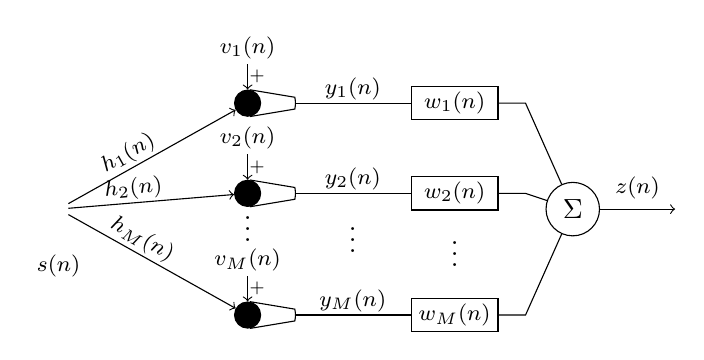
\begin{tikzpicture}
    % Adjustments
    \def\micd{.1cm}                % mic diameter
    \def\micl{.6cm}                % mic length
    \def\micw{.15cm}                % mic width
    \def\micbend{10}               % mic bottom bend
    \def\micdistance{.8cm}         % distance between microphones
    \def\filterdistance{1.9cm}     % distance between microphone and filter
    \def\filteroutline{.9cm}       % length of line which gets out of filter
    \def\sumdistance{1.5cm}        % distance of sum node to the filter
    \def\sumoutline{1cm}           % length of line which gets out of sum
    \def\headdistance{2.4cm}       % distance between microphone and head
    % Styles
    \tikzset{%
      mic head/.style={fill=black,draw=black,circle,minimum size=\micd},
      filter/.style={draw,minimum width=1.1cm,inner sep=2pt},
      sum/.style={draw,circle},
      xlabel/.style={inner sep=1pt,above,midway},
      sumlabel/.style={xlabel},
      hlabel/.style={xlabel,sloped,pos=.4},
      head/.style={font=\Large}
    }%
    % Draw Microphones
    \begin{scope}[start chain=going below,every node/.style={on chain},node distance=\micdistance]
      \node[mic head] (mic1) {};
      \node[mic head] (mic2) {};
      \node[mic head,yshift=-0.5*\micdistance] (mic3) {};
    \end{scope}
    \node[yshift=12pt] at ($(mic2)!.5!(mic3)$) {$\vdots$};
    \foreach \m in {1,2,3} {%
      \coordinate (m1) at ($(mic\m)+(\micl,\micw/2)$);
      \coordinate (m2) at ($(mic\m)+(\micl,-\micw/2)$);
      \draw (tangent cs:node=mic\m,point={(m1)},solution=1) -- (m1) to[bend left=\micbend] (m2) -- (tangent cs:node=mic\m,point={(m2)},solution=2);
    }%
    % Draw Filter
    \foreach \m/\i in {1/1,2/2,3/M} {%
      \node[filter,right=\filterdistance of mic\m] (filter\m) {\footnotesize $w_{\i}(n)$};
      \draw ($(mic\m)+(\micl,0)$) to node[xlabel] (x\m) {\footnotesize $y_{\i}(n)$} (filter\m);
    }%
    \node[yshift=3pt] at ($(filter2)!.5!(filter3)$) {$\vdots$};
    \node[yshift=3pt] at ($(x2)!.5!(x3)$) {$\vdots$};
    % Sum Node %
    \node[sum] (sum) at ($(filter1)!.5!(filter3)+(\sumdistance,0)$) {$\Sigma$};
    \draw[->] (sum) -- node[above] {\footnotesize $z(n)$} ++(1.3,0);
    % Connect filter with sum %
    \foreach \m in {1,2,3} {%
      \draw (filter\m) -- ++(\filteroutline,0) -- (sum);
    }%
    % Head
    \node[head] (head) at ($(mic1)!.5!(mic3)-(\headdistance,0)$) {\PHtattooedHead};
    \node[fill=white,minimum width=4.8pt,minimum height=5.7pt,inner sep=0pt] at ($(head.center)+(2.3pt,-2.5pt)$) {};
    \node at ($(head.center)+(0.0pt,-20.5pt)$) {\footnotesize $s(n)$};
    % Connect head with mics
    \foreach \m/\i in {1/1,2/2,3/M} {%
      \draw[->] (head) -- node[hlabel] {\footnotesize $h_{\i}(n)$} (mic\m);
    }%
    % Draw noise
    \draw[<-] (mic1) -- node[above=0.1cm] {\footnotesize $v_1(n)$} node[right = -0.1cm] {\footnotesize ${}_{+}$} ++(0,0.5);
    \draw[<-] (mic2) -- node[above=0.1cm] {\footnotesize $v_2(n)$} node[right = -0.1cm] {\footnotesize ${}_{+}$} ++(0,0.5);
    \draw[<-] (mic3) -- node[above=0.1cm] {\footnotesize $v_M(n)$} node[right = -0.1cm] {\footnotesize ${}_{+}$} ++(0,0.5);
  \end{tikzpicture}
  \caption{Acoustic system configuration.}
  \label{fig: ac_sys}
\end{figure}
% Denoting the direct path and early reflections of the RIR by $h_{d,m}(n)$ and the late reverberant tail by $h_{r,m}(n)$, the $m$-th microphone signal $x_m(n)$ can also be expressed as
% \begin{equation}
% \label{eq: ysp}
% x_m(n) = \underbrace{h_{d,m}(n) \ast s(n)}_{x_{d,m}(n)} + \underbrace{h_{r,m}(n) \ast s(n)}_{x_{r,m}(n)}, \\
% \end{equation}
% where $x_{d,m}(n)$ is the $m$-th direct speech component and $x_{r,m}(n)$ is the $m$-th late reverberant speech component.
Using the filter-and-sum structure in Fig.~\ref{fig: ac_sys}, the output signal $z(n)$ is equal to the sum of the filtered microphone signals, i.e.,
\begin{align}
  z(n) & = \sum_{m=1}^{M} x_m(n) \ast  w_m(n) \\
  \label{eq: outcomp}
  & = s(n) \ast \underbrace{\sum_{m=1}^{M} h_m(n) \ast  w_m(n)}_{c(n)},
\end{align}
where $w_m(n)$ is the filter applied to the $m$-th microphone signal and $c(n)$ denotes the equalized impulse response (EIR) between the source and the output of the system.
In vector notation, the RIR $\mathbf{h}_m$ and the filter $\mathbf{w}_m$ are given by 
\begin{align}
\mathbf{h}_m  & = [h_m(0) \; h_m(1) \; \ldots \; h_m(L_h-1)]^T, \\
\mathbf{w}_m  & = [w_m(0) \; w_m(1) \; \ldots \; w_m(L_w-1)]^T,
\end{align}
where $L_h$ and $L_w$ denote the RIR length and the filter length, respectively.
Using the $M L_w$--dimensional stacked filter vector $\mathbf{w} = [\mathbf{w}^T_1 \; \mathbf{w}^T_2 \; \ldots \; \mathbf{w}^T_M]^T$, the EIR vector $\mathbf{c}$ of length $L_c = L_h + L_w - 1$, i.e., $\mathbf{c} = [c(0) \; c(1) \; \ldots \; c(L_c-1)]^T$, can be expressed as~\cite{Miyoshi_ITASS_1988, Kodrasi_ITASLP_2013}
\begin{equation}
\label{eq: eir}
\mathbf{c} = \mathbf{H}\mathbf{w},
\end{equation}
with $\mathbf{H}$ the $L_c \times ML_w$--dimensional multi-channel convolution matrix of the RIRs, i.e., $\mathbf{H}  = [\mathbf{H}_1 \; \mathbf{H}_2 \; \ldots \; \mathbf{H}_M]$, and
\begin{equation}
\mathbf{H}_m \! = \! \begin{bmatrix}
    h_m(0) & 0 &  \ldots & 0 \\
    h_m(1) & h_m(0) & \ddots & \vdots \\
    \vdots & h_m(1) & \ddots & 0 \\
    h_m(L_h\!-\!1) & \vdots & \ddots & h_m(0) \\
    0 & h_m(L_h\!-\!1) & \ddots & h_m(1) \\
    \vdots & \ddots & \ddots & \vdots \\
    0 & \ldots & 0 & h_m(L_h\!-\!1)
   \end{bmatrix}.
 \end{equation}
Defining the $L_w$--dimensional $m$-th reverberant signal vector $\mathbf{x}_m(n)$ and the $L_c$--dimensional clean speech vector $\mathbf{s}(n)$ as
\begin{align}
\mathbf{x}_m(n) & = [x_m(n) \; x_m(n-1) \; \ldots \; x_m(n-L_w+1)]^T, \\
\mathbf{s}(n) & = [s(n) \; s(n-1) \; \ldots \; s(n-L_c+1)]^T,
\end{align}
with $\mathbf{x}_m(n) = \mathbf{H}_m^T \mathbf{s}(n)$, the output signal $z(n)$ in~(\ref{eq: outcomp}) can now be expressed as
\begin{equation}
\label{eq: outsig_vec}
z(n) = \sum_{m=1}^M \mathbf{w}_m^T\mathbf{x}_m(n) = \sum_{m=1}^M \mathbf{w}_m^T\mathbf{H}^T_m\mathbf{s}(n) = \underbrace{\mathbf{w}^T\mathbf{H}^T}_{\mathbf{c}^T}\mathbf{s}(n).
\end{equation}
Alternatively,~(\ref{eq: outsig_vec}) can also be expressed as
\begin{equation}
\label{eq: outsig_vecalter}
z(n) = \sum_{m=1}^M \mathbf{x}_m^T(n)\mathbf{w}_m = \mathbf{x}^T(n)\mathbf{w},
\end{equation}
with $\mathbf{x}(n) = [\mathbf{x}^T_1(n) \; \mathbf{x}^T_2(n) \; \ldots \; \mathbf{x}^T_M(n)]^T$ the $ML_w$--dimensional stacked reverberant signal vector.
Based on~(\ref{eq: outsig_vecalter}), the output signal vector $\mathbf{z}(n)$ of length $L_z$, i.e., 
\begin{equation}
\label{out_vec}
\mathbf{z}(n) = [z(n) \; z(n-1) \; \ldots \; z(n-L_z+1)]^T,
\end{equation}
can be written as
\begin{equation}
\label{eq: td_vec}
\mathbf{z}(n) = \mathbf{X}(n)\mathbf{w},
\end{equation}
with $\mathbf{X}(n)$ the $L_z \times ML_w$--dimensional multi-channel convolution matrix of the reverberant signals, i.e.,  $ \mathbf{X}(n) = [\mathbf{X}_1(n) \; \mathbf{X}_2(n) \; \ldots \; \mathbf{X}_M(n)]$, and %
% {{\begin{equation}
% \mathbf{X}_m(n) = \begin{bmatrix}
%     x_m(n) & x_m(n-1) &  \cdots & x_m(n-L_w+ 1) \\
%     x_m(n-1) & x_m(n-2) & \cdots & x_m(n-L_w) \\
%     \vdots & \vdots & \ddots & \vdots \\
%     x_m(n-L_z+1) & x_m(n-L_z) & \cdots & x_m(n-L_w-L_z+2)
%    \end{bmatrix}.
%  \end{equation}}}
\begin{equation}
\mathbf{X}_m(n) = \begin{bmatrix}
    x_m(n) &   \cdots & x_m(n-L_w+ 1) \\
    x_m(n-1) & \cdots & x_m(n-L_w) \\
    \vdots & \ddots & \vdots \\
    x_m(n-L_z+1) & \cdots & x_m(n-L_w-L_z+2)
   \end{bmatrix}.
 \end{equation} %
For conciseness, the time index $n$ will be omitted when possible in the remainder of this paper.

\section{Acoustic Multi-Channel Equalization Techniques}
\label{sec: ame}
Acoustic multi-channel equalization techniques aim at speech dereverberation by designing a filter $\mathbf{w}$ such that the EIR $\mathbf{c}$ in~(\ref{eq: eir}) is equal to a dereverberated target EIR $\mathbf{c}_t$.
However, it should be realized that in practice only the perturbed RIRs $\hat{h}_m$ are available, i.e., $\hat{h}_m = h_m + e_m$, where $e_m$ represents the unknown RIR perturbations arising due to fluctuations~(e.g., temperature or position fluctuations~\cite{Radlovic_ITSA_2000}) or due to the sensitivity of BSI and SSI methods to near-common zeros or interfering noise~\cite{Khong_ICASSP_2008,Haque_SPL_2008,Hu_EUSIPCO_2015}.
Hence, for the filter design, the perturbed convolution matrix $\hat{\mathbf{H}} = \mathbf{H} + \mathbf{E}$ is used, where $\mathbf{E}$ represents the convolution matrix of the RIR perturbations.

In this paper we will focus on state-of-the-art least-squares acoustic multi-channel equalization techniques, i.e., MINT~\cite{Miyoshi_ITASS_1988}, RMCLS~\cite{Lim_ITASLP_2014}, and PMINT~\cite{Kodrasi_ITASLP_2013}, which seek to compute the filter $\mathbf{w}$ as the solution to the system of equations
\begin{equation}
\label{eq: syseq}
\mathbf{W}\hat{\mathbf{H}}\mathbf{w} = \mathbf{W}\mathbf{c}_t,
\end{equation}
with $\mathbf{W}$ an $L_c \times L_c$--dimensional diagonal weighting matrix.
For the considered equalization techniques, the definition of the weighting matrix $\mathbf{W}$ and target EIR $\mathbf{c}_t$ is presented in Tables~\ref{tbl: weighting} and~\ref{tbl: target}, where $\mathbf{I}_c$ denotes the $L_c \times L_c$--dimensional identity matrix, $\tau$ denotes a delay, $L_d$ denotes the length of the direct path and early reflections, and $p \in \{1, \; 2, \; \ldots, \; M \}$.
The delay $\tau$ is incorporated in all techniques in order to relax the causality constraints on the filter design~\cite{Hikichi_EURASIP_2007}.
The length of the direct path and early reflections $L_d$ in the RMCLS and PMINT techniques is typically considered to be between $10$-$50$ ms~\cite{Lim_ITASLP_2014, Kodrasi_ITASLP_2013}.
\begin{table}[b!]
\begin{center}
  \caption{Definition of the weighting matrix $\mathbf{W}$ for state-of-the-art least-squares equalization techniques.}
  \label{tbl: weighting}
  \begin{tabularx}{\linewidth}{Xr}
    \toprule
    Technique & Weighting matrix $\mathbf{W}$ \\
    \midrule
    MINT & {\color{white}{${\rm{diag}}\{[\underbrace{1 \; \ldots \; 1}_{\tau} \; \underbrace{1 \; 0 \; \ldots \; 0}_{L_d} \; 1 \; \ldots 1]^{T}\}$}} $\mathbf{I}_c$\\
    RMCLS & ${\rm{diag}}\{[\underbrace{1 \; \ldots \; 1}_{\tau} \; \underbrace{1 \; 0 \; \ldots \; 0}_{L_d} \; 1 \; \ldots 1]^{T}\}$\\
    PMINT & $\mathbf{I}_c$ \\
    \bottomrule
  \end{tabularx}
\end{center}
\end{table}
\begin{table}[b!]
\begin{center}
  \caption{Definition of the target EIR $\mathbf{c}_t$ for state-of-the-art least-squares equalization techniques.}
  \label{tbl: target}
  \begin{tabularx}{\linewidth}{Xr}
    \toprule
    Technique & Target EIR $\mathbf{c}_t$ \\
    \midrule
    MINT & $[\underbrace{0 \; \ldots \; 0}_{\tau} \; 1 \; 0 \; \ldots \; 0 ]^T$ \\
    RMCLS & $[\underbrace{0 \; \ldots \; 0}_{\tau} \; 1 \; 0 \; \ldots \; 0 ]^T$\\
    PMINT &  $[\underbrace{0\phantom{\rlap{$(L_d-1)$}} \ldots 0 }_{\tau} \underbrace{\hat{h}_p(0) \ldots \hat{h}_p(L_d-1)}_{L_d} 0 \ldots 0 ]^{T}$\\
    \bottomrule
  \end{tabularx}
\end{center}
\end{table}
Based on these definitions of $\mathbf{W}$ and $\mathbf{c}_t$ it can be said that on the one hand, the MINT and PMINT techniques constrain all taps of the EIR (since $\mathbf{W} = \mathbf{I}_c$), which results in a good perceptual speech quality but high sensitivity to RIR perturbations~\cite{Hikichi_EURASIP_2007,Kodrasi_ITASLP_2013}, while on the other hand, the RMCLS technique does not constrain all taps of the EIR (since $\mathbf{W} \neq \mathbf{I}_c$), which results in a lower sensitivity to RIR perturbations but decreased perceptual speech quality~\cite{Lim_ITASLP_2014, Kodrasi_ITASLP_2013}.

For all considered equalization techniques, the filter solving~(\ref{eq: syseq}) is computed by minimizing the least-squares cost function
\begin{equation}
\label{eq: ls_cost}
\boxed{J_{_{\text{LS}}} = \|\mathbf{W} (\hat{\mathbf{H}}\mathbf{w} - \mathbf{c}_t) \|_2^2.}
\end{equation} 
Assuming that the RIRs do not share any common zeros~\cite{Miyoshi_ITASS_1988} and using $L_w \geq \left\lceil{\frac{L_h-1}{M-1}}\right\rceil$~\cite{Harikumar_ITSP_1998}, the least-squares filter solving~(\ref{eq: syseq}) and minimizing~(\ref{eq: ls_cost}) to $0$ is equal to
\begin{equation}
\label{eq: w_ls}
\mathbf{w}_{_{\text{LS}}} = (\mathbf{W}\hat{\mathbf{H}})^+(\mathbf{W}\mathbf{c}_t),
\end{equation}
where $\{ \cdot \}^+$ denotes the matrix pseudo-inverse. 
When the true RIRs are available, i.e., $\hat{\mathbf{H}} = \mathbf{H}$, the least-squares filter yields perfect dereverberation, i.e., $\mathbf{W}\mathbf{H}\mathbf{w}_{_{\text{LS}}} = \mathbf{W}\mathbf{c}_t$~\cite{Hacihabibouglu_ITASLP_2012,Kodrasi_ITASLP_2013}.
However, in the presence of RIR perturbations, i.e., $\hat{\mathbf{H}} \neq \mathbf{H}$, the least-squares filter typically fails to achieve dereverberation, i.e., $\mathbf{W}\mathbf{H}\mathbf{w}_{_{\text{LS}}} \neq \mathbf{W}\mathbf{c}_t$, possibly causing severe distortions in the output signal~\cite{Kodrasi_ITASLP_2013}.

\section{Regularized Acoustic Multi-Channel Equalization Techniques}
\label{sec: reg}
In order to increase the robustness of acoustic multi-channel equalization techniques against RIR perturbations, it has been proposed to incorporate regularization in the filter design, such that the energy of distortions due to RIR perturbations is reduced~\cite{Hikichi_EURASIP_2007,Kodrasi_ITASLP_2013}.
Regularized equalization techniques design filters by minimizing the regularized least-squares cost function
\begin{equation}
\label{eq: rls_cost}
\boxed{J_{_{\text{RLS}}} = \|\mathbf{W}(\hat{\mathbf{H}}\mathbf{w} - \mathbf{c}_t) \|_2^2 + \delta \mathbf{w}^T\mathbf{R}_e\mathbf{w},}
\end{equation}
where the matrix $\mathbf{R}_e$ models ${\cal{E}} \{\mathbf{E}^T\mathbf{E}\}$, with ${\cal{E}}$ the expected value operator, and $\delta$ is a regularization parameter providing a trade-off between the least-squares error and the distortion energy due to RIR perturbations.
When knowledge is available about the type of RIR perturbations (e.g., arising due to microphone position fluctuations or arising from BSI or SSI methods), the matrix $\mathbf{R}_e$ can be constructed based on an appropriate perturbation model~\cite{Jungmann_ITASLP_2012, Lim_IWAENC_2014}.
When such knowledge is not available, the RIR perturbations are often assumed to be spatially and temporally white, i.e., $\mathbf{R}_e = \mathbf{I}_w$, with $\mathbf{I}_w$ denoting the $ML_w \times ML_w$--dimensional identity matrix~\cite{Hikichi_EURASIP_2007,Kodrasi_ITASLP_2013}.
This assumption has been used for the regularized techniques in Section~\ref{sec: reg_spa}.

Minimizing~(\ref{eq: rls_cost}) yields the regularized least-squares filter
\begin{equation}
\label{eq: w_rls}
\mathbf{w}_{_{\text{RLS}}} = [ (\mathbf{W}\hat{\mathbf{H}})^T(\mathbf{W}\hat{\mathbf{H}}) + \delta \mathbf{R}_{e} ]^{-1}(\mathbf{W}\hat{\mathbf{H}})^T(\mathbf{W}\mathbf{c}_t).
\end{equation}
While the least-squares filter in~(\ref{eq: w_ls}) typically fails to achieve dereverberation in the presence of RIR perturbations, it has been experimentally validated in~\cite{Kodrasi_ITASLP_2013} that the regularized least-squares filter in~(\ref{eq: w_rls}) results in a significantly better performance.
However, as can be seen from~(\ref{eq: rls_cost}), the regularization term is signal-independent, since it only depends on an RIR perturbation model and does not incorporate any knowledge about the output signal.

\section{Sparsity-Promoting Acoustic Multi-Channel Equalization Techniques}
\label{sec: spa}
Instead of using a signal-independent regularization term, in this section we propose to increase the robustness of equalization techniques by incorporating a signal-dependent penalty function in the filter design, enforcing the output signal $z(n)$ to exhibit spectro-temporal characteristics of a clean speech signal.
While in principle any penalty function imposing a well-defined characteristic of clean speech could be used, we propose to use penalty functions which promote sparsity of the output signal in the STFT domain.
The advantage of promoting sparsity of the STFT coefficients of the output signal is expected to be twofold.
First, it is widely accepted that clean speech is sparse in the STFT domain~\cite{makino_2010,Tashev_IWAENC_2010,Gerkmann_IWAENC_2010}. 
Empirical observations, e.g., in~\cite{makino_2010}, have shown that when clean speech is corrupted by reverberation, the STFT coefficients of the mixture are less sparse than the STFT coefficients of clean speech (cf. Figs.~\ref{fig: spec}(a) and (b)).
Hence, promoting sparsity of the STFT coefficients of the output signal can yield a signal which better resembles a clean speech signal.
Second, in the presence of RIR perturbations, non-robust equalization techniques introduce distortions (i.e., non-zero STFT coefficients) in the output signal~\cite{Kodrasi_ITASLP_2013} (cf. Fig.~\ref{fig: spec}(c)).
By promoting sparsity of the STFT coefficients of the output signal, it is expected that these distortions are suppressed.
In the remainder of this section, the proposed signal-dependent least-squares cost function is formulated, several possible sparsity-promoting penalty functions are discussed, and the iterative method for optimizing this cost function is presented. 

It should be noted that sparsity-promoting techniques have also been proposed to increase the robustness of BSI methods to additive noise~\cite{Lin_Neural_2008,Kowalczyk_SPL_2013}.
    However, unlike the sparsity-promoting equalization techniques proposed in the following which aim at enforcing sparsity on the output speech signal, sparsity-promoting techniques for BSI aim at enforcing sparsity on the estimated RIRs.

\subsection{Sparsity-promoting cost function}
In order to incorporate the STFT of the output signal in the filter design, the STFT coefficients $Z(k,l)$ of the output signal $z(n)$ are computed as
\begin{equation}
  \label{eq: stft}
Z(k,l) = \sum_{n=0}^{N-1}w_{_{\text{STFT}}}(n)z(lR+n)e^{-\frac{j 2 \pi k n}{N}},
\end{equation}
where $w_{_{\text{STFT}}}(n)$ denotes the STFT analysis window of length $N$, $k = 0, \; 1, \; \ldots, \; N-1$, denotes the frequency bin index, $l = 0, \; 1, \; \ldots, \; L-1$, denotes the frame index with $L$ the total number of frames,  and $R$ denotes the frame shift.
Based on~(\ref{eq: stft}), we define the STFT operator $\mathbf{\Psi} \in {\cal{C}}^{NL \times L_z}$ similarly as in~\cite{Kowalski_ITASLP_2010,Arberet_ITASLP_2013}, transforming the $L_z$--dimensional time domain vector $\mathbf{z}$ in~(\ref{out_vec}) into the $NL$--dimensional time-frequency domain vector $\tilde{\mathbf{z}}$, i.e.,
\begin{equation}
\label{eq: tilde_z}
\tilde{\mathbf{z}} = \mathbf{\Psi}\mathbf{z}.
\end{equation}
In other words, the vector $\tilde{\mathbf{z}}$ consists of all STFT coefficients $Z(k,l)$, $k = 0, \; 1, \; \ldots, \; N-1$, $l = 0, \; 1, \; \ldots, \; L-1$.
Using~(\ref{eq: td_vec}), the time-frequency domain vector $\tilde{\mathbf{z}}$ can be expressed in terms of the filter $\mathbf{w}$ as
\begin{equation}
\tilde{\mathbf{z}} = \mathbf{\Psi}\mathbf{X}\mathbf{w}.
\end{equation}
It should be noted that for a tight analysis window $w_{_{\rm STFT}}(n)$, i.e., the same window can be used as a synthesis window such that the perfect overlap-add constraint is satisfied, the inverse short-time Fourier transform operator $\mathbf{\Psi}^{H} \in {\cal{C}}^{L_z \times NL}$ satisfies $\mathbf{\Psi}^{H}\mathbf{\Psi} = \mathbf{I}_z$, with $\mathbf{I}_z$ the $L_z \times L_z $--dimensional identity matrix.

Aiming at promoting sparsity of the STFT coefficients of the output signal in the filter design, we now propose to add a signal-dependent term to the least-squares cost function, i.e.,
\begin{empheq}[box=\fbox]{align}
\label{eq: cost_sp1}
J_{_{\text{SLS}}} & = J_{_{\text{LS}}} + \eta f_{_{\text{SP}}}(\tilde{\mathbf{z}}) \\
\label{eq: cost_sp2}
  & = \|\mathbf{W}(\hat{\mathbf{H}}\mathbf{w}-\mathbf{c}_t) \|_2^2 + \eta f_{_{\text{SP}}}(\boldsymbol{\Psi}\mathbf{X}\mathbf{w}),
\end{empheq}
with $f_{_{\text{SP}}}$ a sparsity-promoting penalty function (cf. Section~\ref{sec: fsp}) and $\eta$ a weighting parameter providing a trade-off between the minimization of the least-squares error and the value of the penalty function.

\subsection{Sparsity-promoting penalty functions}
\label{sec: fsp}
In this paper we will consider three commonly used sparsity-promoting norms for the penalty function $f_{_{\text{SP}}}$ in~(\ref{eq: cost_sp2}), i.e., the $l_0$-norm\footnote{Note that the $l_0$-norm is not a norm in the strict mathematical sense, since it does not satisfy all the norm properties.}, the $l_1$-norm, and the weighted $l_1$-norm\cite{Natarajan_SIAM_1995,Boyd_book,Chartrand_ICASSP_2014,Candes_FA_2008}. 

The $l_0$-norm $f_{_{\text{SP}}}^0(\tilde{\mathbf{z}})$ counts the number of non-zero entries in $\tilde{\mathbf{z}}$, i.e.,
\begin{equation}
\label{eq: lo_norm}
f_{_{\text{SP}}}^0(\tilde{\mathbf{z}}) = \| \tilde{\mathbf{z}}\|_0 = |q: \tilde{z}(q) \neq 0|.
\end{equation}
Using $f_{_{\text{SP}}}^0(\tilde{\mathbf{z}})$ in~(\ref{eq: cost_sp2}) penalizes the non-zero STFT coefficients of the output signal, which can be advantageous to suppress the reverberant energy as well as the distortions introduced by non-robust least-squares equalization techniques.
% In the presence of reverberation, the pauses between phonemes and the formant transitions in voiced sounds, i.e., the (nearly) zero energy STFT coefficients of the clean speech signal, are filled with reverberant energy.
% In addition, in the presence of RIR perturbations, non-robust acoustic multi-channel equalization techniques introduce additional distortions (i.e., additional non-zero STFT coefficients) in the output speech signal.
% In order to increase the robustness of acoustic multi-channel equalization techniques against RIR perturbations and obtain an output speech signal that better resembles a clean speech signal, one possibility is to minimize the number of non-zero coefficients in $\tilde{\mathbf{z}}$, which can be achieved by using an $l_0$-norm\footnote{Note that the $l_0$-norm is not a norm in the mathematical sense, since it does not satisfy all the norm properties.} penalty function, i.e.,
% \begin{equation}
% \label{eq: lo_norm}
% f_{_{\text{SP}}}^0(\tilde{\mathbf{z}}) = \| \tilde{\mathbf{z}}\|_0 = |i: \tilde{z}(i) \neq 0|.
% \end{equation}
However, the $l_0$-norm is non-convex, and it is well known that optimization problems with non-convex penalty functions are typically hard (if not impossible) to solve, particularly for large scale problems~\cite{Natarajan_SIAM_1995}.
In addition, iterative methods proposed to solve such optimization problems are not guaranteed to converge to the global minimum, but only to a local minimum~\cite{Nocedal_book}. 

%However, it has been shown that non-convex penalty functions can result in a more sparse solution than convex ones~\cite{Chartrand_ICASSP_2008}.
A commonly used alternative to the $l_0$-norm is the $l_1$-norm penalty function $f_{_{\text{SP}}}^1(\tilde{\mathbf{z}})$, defined as
\begin{equation}
  \label{eq: l1_norm}
  f_{_{\text{SP}}}^1(\tilde{\mathbf{z}}) = \| \tilde{\mathbf{z}}\|_1 = \sum_{q = 0}^{NL-1} |\tilde{z}(q)|.
\end{equation}
The $l_1$-norm can be viewed as a convex relaxation of the $l_0$-norm, and efficient methods have been proposed to solve optimization problems with $l_1$-norm penalty functions~\cite{Chartrand_ICASSP_2014,Boyd_book}.
As can be seen in~(\ref{eq: l1_norm}), the $l_1$-norm is magnitude-dependent, differing from the $l_0$-norm by penalizing the coefficients of $\tilde{\mathbf{z}}$ with larger magnitude more than the coefficients with smaller magnitude.
This penalization is not necessarily desirable, since it does not guarantee the preservation of the spectro-temporal structure of a typical speech signal. 

% Furthermore, it has been shown that under certain conditions, replacing the $l_0$-norm by the $l_1$-norm provides the solution to the original $l_0$-norm optimization problem~\cite{Candes_IT_2005,Donoho_IT_2006}. 
% In practice however, the $l_1$-norm relaxation is very often used when these conditions are not satisfied, typically resulting in a solution which does not optimize the original $l_0$-norm optimization problem, but nevertheless provides smaller $l_0$-norm values.
To counteract the magnitude dependency of the $l_1$-norm, the weighted $l_1$-norm penalty function $f_{_{\text{SP}}}^{w,1}(\tilde{\mathbf{z}})$ has been proposed~\cite{Candes_FA_2008}, defined as
\begin{equation}
\label{eq: wl1_norm}
f_{_{\text{SP}}}^{w,1}(\tilde{\mathbf{z}}) = \|{\rm diag}\{\mathbf{u} \}\tilde{\mathbf{z}}\|_1 = \sum_{q = 0}^{NL-1} |u(q) \tilde{z}(q)|,
\end{equation}
with $\mathbf{u}$ an $NL$--dimensional vector of positive scalar weights, i.e., $u(q) > 0$, $q = 0, \; 1, \; \ldots, \; NL-1$,
% Using $u(q) = 1$, $q = 0, \; \ldots, \; NL-1$, yields the standard $l_1$-norm penalty function in~(\ref{eq: l1_norm}).
% The weighted $l_1$-norm penalty function
selectively penalizing the coefficients of $\tilde{\mathbf{z}}$.
To promote the same sparsity structure in the output signal as in the desired signal, it has been proposed in~\cite{Candes_FA_2008} to select the weighting vector such that it has small values when the desired signal has non-zero magnitude and significantly larger values otherwise.
% Replacing the $l_1$-norm by a weighted $l_1$-norm has been shown to enhance sparsity and improve the performance in sparse signal recovery applications~\cite{Candes_FA_2008,Friedlander_IEEEIT_2012}.
In the context of speech dereverberation, it would hence be desirable to select the weights to be inversely proportional to the magnitude of the STFT coefficients of the clean speech signal, i.e., 
\begin{equation}
\label{eq: ws}
u(q) = \frac{1}{|\tilde{s}(q)| }, \; \; \; \; q = 0, \; 1, \; \ldots, \; NL-1,
\end{equation}
with $\tilde{s}(q)$ the STFT coefficients of the clean speech signal computed similarly as in~(\ref{eq: tilde_z}).
Using the weights in~(\ref{eq: ws}) results in a larger penalization - and hence, a larger suppression - of the STFT coefficients of the output signal corresponding to the STFT coefficients of the clean speech signal with a small magnitude.
However, since the clean speech signal is obviously not available, we propose to use one of the reverberant microphone signals and compute the weights as
\begin{equation}
\label{eq: weights}
u(q) = \frac{1}{|\tilde{x}_p(q)| + \zeta}, \; \; \; \; q = 0, \; 1, \; \ldots, \; NL-1,
\end{equation}
with $\tilde{x}_p(q)$ the STFT coefficients of the $p$-th microphone signal computed similarly as in~(\ref{eq: tilde_z}) and $\zeta > 0$ a small positive scalar included to avoid division by $0$ and to ensure stability of the weighted $l_1$-norm sparsity-promoting techniques.
When $|\tilde{x}_p(q)| \approx 0$, e.g., during speech absence, using $\zeta$ ensures that $u(q)$ is large but finite, such that the magnitude of the STFT coefficients of the reconstructed signal is also (nearly) $0$.
% As already mentioned, the key difference between the $l_1$- and $l_0$-norms is the magnitude dependence, i.e., the larger coefficients are penalized more heavily than the smaller coefficients in the $l_1$-norm, while a more equal penalization arises in the $l_0$-norm.
% The choice of appropriate weights $u(i)$ can now be used to counteract the magnitude dependency of the $l_1$-norm and to better mimic the $l_0$-norm~\cite{Candes_FA_2008}.
As will be experimentally shown in Section~\ref{sec: robust_increase}, incorporating the weighted $l_1$-norm penalty function using the weights in~(\ref{eq: weights}) typically yields a better dereverberation performance than incorporating the $l_0$- or $l_1$-norm penalty functions.
The advantage of using the weighted $l_1$-norm penalty function lies in the fact that appropriate weights as in (\ref{eq: weights}) ensure that the spectro-temporal structure of a typical speech signal is preserved.

\subsection{Iterative optimization method}
Since no closed-form expression is available for the filter minimizing the sparsity-promoting cost function in~(\ref{eq: cost_sp2}), iterative optimization methods are required.
We propose to use the ADMM~\cite{Boyd_admm_2011}, since it is a well-suited method for solving large scale optimization problems of the form in~(\ref{eq: cost_sp2}).
Within the ADMM framework, the minimization of the sparsity-promoting cost function in~(\ref{eq: cost_sp2}) is reformulated as
\begin{equation}
\label{eq: cost_reform}
\min_{\mathbf{w}} \left[ \|\mathbf{W}(\hat{\mathbf{H}}\mathbf{w}-\mathbf{c}_t) \|_2^2 + \eta f_{_{\text{SP}}}(\tilde{\mathbf{a}}) \right] \; \; {\text{subject to}} \; \; \boldsymbol{\Psi}\mathbf{X}\mathbf{w} = \tilde{\mathbf{a}},
\end{equation}
where the $NL$--dimensional auxiliary variable $\tilde{\mathbf{a}}$ is introduced such that the optimization problem in~(\ref{eq: cost_sp2}) can be split into simpler sub-problems.
The augmented Lagrangian of~(\ref{eq: cost_reform}) is equal to
\begin{equation}
\label{eq: lag}
{\cal{L}} = \|\mathbf{W}(\hat{\mathbf{H}}\mathbf{w}-\mathbf{c}_t) \|_2^2 + \eta f_{_{\text{SP}}}(\tilde{\mathbf{a}}) + \frac{\rho}{2} \|\boldsymbol{\Psi}\mathbf{X}\mathbf{w} +\boldsymbol{\lambda} - \tilde{\mathbf{a}}\|_2^2,
\end{equation}
with $\boldsymbol{\lambda}$ the $NL$--dimensional dual (splitting) variable and $\rho>0$ the ADMM penalty parameter.
ADMM minimizes~(\ref{eq: lag}) alternately with respect to the variables $\mathbf{w}$ and $\tilde{\mathbf{a}}$, followed by a dual ascent over the variable $\boldsymbol{\lambda}$~\cite{Boyd_admm_2011}.
The ADMM update rules are given by
\begin{align}
\label{eq: upw}
\begin{split}
\mathbf{w}^{(i+1)} & = \underset{\mathbf{w}}{\arg\min} \left[ \|\mathbf{W}(\hat{\mathbf{H}}\mathbf{w} - \mathbf{c}_t)\|_2^2  \right. \\
&\quad \quad \quad \quad \quad + \left.\frac{\rho}{2} \|\mathbf{\Psi}\mathbf{X}\mathbf{w} + \boldsymbol{\lambda}^{(i)} - \tilde{\mathbf{a}}^{(i)} \|_2^2 \right],
\end{split} \\
\label{eq: upz}
\tilde{\mathbf{a}}^{(i+1)} & = \underset{\tilde{\mathbf{a}}}{\arg\min} \left[ \eta f_{_{\text{SP}}}(\tilde{\mathbf{a}}) + \frac{\rho}{2} \|\mathbf{\Psi}\mathbf{X}\mathbf{w}^{(i+1)} + \boldsymbol{\lambda}^{(i)} - \tilde{\mathbf{a}} \|_2^2 \right], \\
\label{eq: up_lambda_sls}
\boldsymbol{\lambda}^{(i+1)} & \!=\! \boldsymbol{\lambda}^{(i)} \!+\! \mathbf{\Psi}\mathbf{X}\mathbf{w}^{(i+1)} \!-\! \tilde{\mathbf{a}}^{(i+1)},
\end{align}
where $\{\cdot\}^{(i)}$ denotes the variable in the $i$-th iteration.
The minimization problem in~(\ref{eq: cost_sp2}) is hence decomposed into simpler sub-problems, which are solved in an alternating fashion using the update rules in~(\ref{eq: upw}),~(\ref{eq: upz}), and~(\ref{eq: up_lambda_sls}) until a termination criterion is satisfied~(cf. Section~\ref{sec: acsys}).
In the following, the update rules for the filter in~(\ref{eq: upw}) and for the auxiliary variable in~(\ref{eq: upz}) are presented.

{\textit{Filter update rule:}} \enspace In order to derive the filter update rule, the gradient of~(\ref{eq: upw}) is set to $\mathbf{0}$, yielding 
\begin{align}
\label{eq: w_admm_sls0}
\begin{split}
\mathbf{w}^{(i+1)} & = [ \underbrace{2 (\mathbf{W}\hat{\mathbf{H}})^T(\mathbf{W}\hat{\mathbf{H}}) + \rho \mathbf{X}^T \mathbf{X}}_{\mathbf{C}} ]^{-1} \\
 &\quad \times [\underbrace{2 (\mathbf{W}\hat{\mathbf{H}})^T (\mathbf{W}\mathbf{c}_t)}_{\mathbf{b}^{}_1} + \rho \underbrace{\mathbf{X}^T \mathbf{\Psi}^H \!(\tilde{\mathbf{a}}^{(i)} - \boldsymbol{\lambda}^{(i)})}_{\mathbf{b}_2^{(i)}}]
\end{split} \\
\label{eq: w_admm_sls}
 & = \mathbf{C}^{-1} (\mathbf{b}_1 + \rho \mathbf{b}_2^{(i)}),
\end{align}
where the variables $\mathbf{C}$, $\mathbf{b}_1$, and $\mathbf{b}_2$ are introduced to highlight the fact that only the variable $\mathbf{b}_2$ is iteration-dependent, whereas the variables $\mathbf{C}$ and $\mathbf{b}_1$ can be pre-computed.
Although~(\ref{eq: w_admm_sls}) appears to require a matrix inversion in each iteration of the ADMM, the filter update can be efficiently computed by, e.g., storing the LU-factorization of $\mathbf{C}$ and using forward and backward substitution~\cite{Golub_Matrix_book}.

{\textit{Auxiliary variable update rule:}} \enspace The auxiliary variable update rule in~(\ref{eq: upz}) is given by the proximal mapping of the sparsity-promoting penalty function~\cite{Chartrand_ICASSP_2014,parikh2014proximal}. The proximal mapping for the $l_0$-, $l_1$-, and weighted $l_1$-norm penalty functions exists in closed-form~\cite{Chartrand_ICASSP_2014,parikh2014proximal}, enabling to efficiently compute the auxiliary variable update rule in each iteration of the ADMM.
Simplifying the notation by defining the operator $\left(T \right)_{+} = \max (T,0)$ and the variable $\mathbf{b}$ as
\begin{equation}
\mathbf{b}^{(i)}= \mathbf{\Psi}\mathbf{X}\mathbf{w}^{(i+1)} + \boldsymbol{\lambda}^{(i)},
\end{equation} 
the proximal mapping for the penalty functions $f_{_{\text{SP}}}^0$, $f_{_{\text{SP}}}^1$, and $f_{_{\text{SP}}}^{w,1}$ is given by the following element-wise mappings
\begin{equation}
  \label{eq: aux_update}
   \tilde{a}^{(i+1)}(q) =
  \begin{cases}
   \left(\left|b^{(i)}(q)\right| - \frac{\eta}{\rho} \right)_+ \frac{ b^{(i)}(q) }{ \left|b^{(i)}(q)\right| - \frac{\eta}{\rho} } & \text{if } f_{_{\text{SP}}}^0 \\ \\
   \left( \left|b^{(i)}(q)\right| - \frac{\eta}{\rho} \right)_+\frac{b^{(i)}(q)}{\left|b^{(i)}(q)\right|} & \text{if } f_{_{\text{SP}}}^1 \\ \\
   \left( \left|b^{(i)}(q)\right| - \frac{\eta}{\rho}u(q) \right)_+\frac{b^{(i)}(q)}{\left|b^{(i)}(q)\right|} & \text{if } f_{_{\text{SP}}}^{w,1}
   \end{cases}.
  \end{equation}
  As can be observed in~(\ref{eq: aux_update}), the mapping for the $l_0$-norm penalty function reduces the $l_0$-norm of the auxiliary variable $\tilde{\mathbf{a}}$ in each iteration of the ADMM by changing all but the largest elements (with magnitude larger than $\frac{\eta}{\rho}$) to $0$.
  The mapping for the $l_1$-norm penalty function reduces the $l_1$-norm of $\tilde{\mathbf{a}}$ in each iteration by subtracting $\frac{\eta}{\rho}$ from the magnitude of every element of $\tilde{\mathbf{a}}$.
  Finally, the mapping for the weighted $l_1$-norm penalty function is similar to the mapping for the $l_1$-norm, with the only difference consisting in the multiplication of the threshold $\frac{\eta}{\rho}$ with the weights $u(q)$. 

% The proximal mapping for these penalty functions is presented in the following, where the variable 
% is defined to simplify the notation. \newline
% The proximal mapping for the $l_0$-norm penalty function $f_{_{\text{SP}}}^0$ is the element-wise {\textit{hard thresholding}} map, i.e.,
% with $\left(T \right)_{+} = \max (T,0)$.
% Hard-thresholding uses a non-linear operator to reduce the $l_0$-norm of $\tilde{\mathbf{a}}$ in each iteration of the ADMM algorithm by changing all but the largest elements (larger than $\frac{\eta}{\rho}$) to $0$. \newline
% The proximal mapping for the $l_1$-norm penalty function $f_{_{\text{SP}}}^1$ is the element-wise {\textit{soft thresholding}} map, i.e.,
% Soft-thresholding reduces the $l_1$-norm of $\tilde{\mathbf{a}}$ in each iteration of the ADMM algorithm by subtracting $\frac{\eta}{\rho}$ from the magnitude of every element of $\tilde{\mathbf{a}}$. \newline
% The proximal mapping for the weighted $l_1$-norm penalty function $f_{_{\text{SP}}}^{w,1}$ is similar to the soft-thresholding in~(\ref{eq: aux_up_l1}), with the only difference consisting in the multiplication of the soft threshold with the weights in $\mathbf{u}$, i.e.,
% , weighted soft-thresholding reduces the $l_1$-norm of $\tilde{\mathbf{a}}$ in each iteration of the ADMM algorithm by subtracting $\frac{\eta}{\rho} u(q)$ from the magnitude of every element of $\tilde{\mathbf{a}}$. \newline
  In summary, using the filter update rule in~(\ref{eq: w_admm_sls0}), the auxiliary variable update rule in~(\ref{eq: aux_update}) depending on the used sparsity-promoting penalty function, and the dual variable update rule in~(\ref{eq: up_lambda_sls}), the sparsity-promoting least-squares filters can be iteratively computed until a termination criterion is satisfied (cf. Section~\ref{sec: acsys}).
  
\section{Simulation Results}
\label{sec: exp}
In this section the performance of the proposed sparsity-promoting acoustic multi-channel equalization techniques is investigated by means of instrumental measures.
In Section~\ref{sec: acsys} the considered acoustic systems, algorithmic settings, and instrumental measures are introduced.
In Section~\ref{sec: robust_increase} the robustness against RIR perturbations for the MINT, RMCLS, and PMINT techniques when incorporating different sparsity-promoting penalty functions is investigated.
In Section~\ref{sec: wl1} the performance of the weighted $l_1$-norm sparsity-promoting techniques is compared for all considered acoustic systems and RIR perturbation levels.
In Section~\ref{sec: eta_rho} the performance of the weighted $l_1$-norm sparsity-promoting PMINT technique for different choices of the weighting and penalty parameters $\eta$ and $\rho$ is investigated.
Finally, in Section~\ref{sec: reg_spa} the performance of the signal-dependent weighted $l_1$-norm sparsity-promoting PMINT technique is compared to the performance of the signal-independent regularized PMINT technique.
% While simulated acoustic systems and simulated RIR perturbations have been used in Sections~\ref{sec: robust_increase} to \ref{sec: reg_spa}, in Section~\ref{sec: real_ssi} the performance of the weighted $l_1$-norm sparsity-promoting PMINT technique is investigated for a measured acoustic system and RIR perturbations arising from least-squares SSI~\cite{Lim_ITASLP_2014}.
Exemplary sound samples from each simulation can be found at \url{http://bit.ly/2cPDnsN}.
\subsection{Acoustic systems, algorithmic settings, and instrumental measures}
\label{sec: acsys}
\vskip 5pt
\textit{Acoustic systems} 
\vskip 5pt
We have considered three different reverberant acoustic systems with a single speech source and $M=4$ omni-directional microphones.
The RIRs between the speech source and the microphones are measured using the swept-sine technique~\cite{Farina_2000} and the reverberant signals are generated by convolving $10$ sentences (approximately $17$ s long) from the HINT database~\cite{Nilsson_JASA_1994} with the measured RIRs.
For each acoustic system, Table~\ref{tbl: ac_sys} presents the reverberation time $T_{60}$ of the room, the source-microphone distance $d_{\text{sm}}$, the inter-microphone distance $d_{\text{im}}$, and the length of the RIRs $L_h$ at a sampling frequency $f_{s} = 8$ kHz.

\begin{table}[t!]
\begin{center}
  \caption{Characteristics of the considered measured acoustic systems.}
  \label{tbl: ac_sys}
  \begin{tabularx}{\linewidth}{Xrrrr}
    \toprule
    Acoustic system & $T_{60}$ [ms] & $d_{\text{sm}}$ [m] & $d_{\text{im}}$ [m] & $L_h$  \\
    \midrule
    $\text{S}_1$ & $610$ & $2$ & $0.04$ & $5000$ \\
    $\text{S}_2$ & $450$ & $3$ & $0.05$ & $3800$ \\
    $\text{S}_3$ & $360$ & $2$ & $0.04$ & $3000$ \\
    \bottomrule
  \end{tabularx}
\end{center}
\end{table}
In order to simulate RIR perturbations, the measured RIRs are perturbed by proportional Gaussian distributed errors as proposed in~\cite{Zhang_HINDAWI_2008}, such that a desired level of normalized projection misalignment~(NPM), i.e.,
\begin{equation}
{\text{NPM}} = 20 \log_{10} \frac{ \left\| \mathbf{h} - \frac{\mathbf{h}^T\hat{\mathbf{h}}}{\hat{\mathbf{h}}^T\hat{\mathbf{h}}}\hat{\mathbf{h}}\right\|_2}{\left\| \mathbf{h} \right\|_2},
\end{equation}
is generated.
Introducing proportional Gaussian distributed errors is a widely used technique to systematically simulate RIR perturbations.
The considered NPMs for each acoustic system are
\begin{equation}
\label{eq: npm}
{\text{NPM}} \in \{ -33~{\rm dB}, \; -27~{\rm dB}, \; \ldots, \; -3~{\rm dB} \},
\end{equation}
with $-33$ dB a moderate perturbation level and $-3$ dB a rather large perturbation level.
The reported NPM values achieved by state-of-the-art BSI methods (for relatively short RIRs) range between $-10$ dB and $-20$ dB~\cite{Hu_EUSIPCO_2015}, hence, the values in~(\ref{eq: npm}) can be considered as rather realistic.
% \vskip 5pt
% \noindent \textit{Measured acoustic system} 
% \vskip 5pt
% \noindent To investigate the performance in a more realistic acoustic scenario we have also considered a recorded acoustic system with reverberation time $T_{60} \approx 450$ ms and $M = 4$ omni-directional microphones.
% The source-microphone distance is $2$ m and the inter-microphone distance is $0.025$ m. 
% The received microhpone signals $\mathbf{y}_m$ are recorded by playing back a clean speech signal from the HINT database over a loudspeaker. 
% The recorded signals contain not only the reverberant signal $\mathbf{x}_m$, but also ambient noise as well as microphone self-noise $\mathbf{v}_m$.
% The broadband speech-to-ambient noise ratio is $25$ dB. \newline
% The true RIRs $\mathbf{h}_m$ are measured using the swept-sine technique, with the RIR length $L_h = 4000$ at a sampling frequency $f_s = 8$ kHz.\footnote{Please note that referring to the measured RIRs as the true RIRs is not entirely correct. The RIRs are measured at a different time instant than the recorded speech, hence, environmental conditions (such as temperature) may have changed, possibly yielding a different true RIR.}
% Furthermore, estimates of the RIRs $\hat{\mathbf{h}}_m$ are obtained using SSI by minimizing the least-squares cost function~\cite{Lim_ITASLP_2014}
% \begin{equation}
% \label{eq: ssi}
% J = \|\mathbf{S}\mathbf{h}_m - \mathbf{y}_m\|_2^2, \; \; \; \; m = 1, \; \ldots, \; M,
% \end{equation}
% where $\mathbf{S}$ denotes the $L_s \times L_h$--dimensional convolution matrix of the clean speech signal, with $L_s = 18 f_s$.
% The minimization of~(\ref{eq: ssi}) yields
% \begin{equation}
% \hat{\mathbf{h}}_m = (\mathbf{S}^T\mathbf{S})^{-1}\mathbf{S}^T\mathbf{y}_m, \; \; \; \; m = 1, \; \ldots, \; M.
% \end{equation}
% Due to the noise in $\mathbf{y}_m$, the estimated RIRs $\hat{\mathbf{h}}_m$ differ from the true RIRs $\mathbf{h}_m$~\cite{Lim_ITASLP_2014}, i.e.,
% \begin{equation}
% \hat{\mathbf{h}}_m = \mathbf{h}_m + (\mathbf{S}^T\mathbf{S})^{-1}\mathbf{S}^T\mathbf{v}_m
% \end{equation}

\vskip 5pt
\textit{Algorithmic settings} 
\vskip 5pt

For all considered equalization techniques the filter length is set to $L_w =\left\lceil{\frac{L_h-1}{M-1}}\right\rceil$, i.e., $L_w = 1667$ for $\text{S}_1$, $L_w = 1267$ for $\text{S}_2$, and $L_w = 1000$ for $\text{S}_3$.
The length of the direct path and early reflections is set to $L_d = 0.01 \times f_s$, i.e., $10$ ms, and the delay is set to $\tau = 90$ (cf. Tables~\ref{tbl: weighting} and~\ref{tbl: target}).
The target EIR $\mathbf{c}_t$ for the PMINT technique is constructed using the first RIR, i.e., $p = 1$ (cf. Table~\ref{tbl: target}).

For the sparsity-promoting filters the STFT is computed using a $32$~ms Hamming window (i.e., $N = 256$) with $50$\% overlap between successive frames.
In order to reduce the computational complexity, the sparsity-promoting filters are computed using only the first two sentences of the reverberant signals~(i.e., $L = 208$), but the complete output signal has been used for the evaluation.
For the weighted $l_1$-norm penalty function, the weights in~(\ref{eq: weights}) are computed using the first microphone signal, i.e., $p=1$, and $\zeta = 10^{-8}$.
The termination criterion for the ADMM is a maximum number of iterations $i_{\max} = 500$.
Since the initialization of the ADMM may influence the resulting sparsity-promoting filter for the non-convex $l_0$-norm penalty function, we have investigated three different initializations of the filter $\mathbf{w}$: 
\begin{itemize}
\item[i)] $\mathbf{w}^{(0)} = [1 \; 0 \; \ldots \; 0]^T$, i.e., the filter yielding the first microphone signal,
\item[ii)] $\mathbf{w}^{(0)}$ is randomly initialized with normally distributed coefficients, 
\item[iii)] $\mathbf{w}^{(0)} = \mathbf{w}_{_{\text{LS}}}$, i.e., the filter resulting from the least-squares techniques.
\end{itemize}
In all simulations we observed that using the filter initialization i), i.e., $\mathbf{w}^{(0)} = [1 \; 0 \; \ldots \; 0]^T$, resulted in the best performance, and hence, the following simulation results are generated using this filter initialization. 

Finally, we have considered several regularization parameters $\delta$ for the regularized techniques and several weighting and penalty parameters $\eta$ and $\rho$ for the sparsity-promoting techniques, i.e.,
\begin{equation}
\label{eq: pars}
\delta, \eta, \rho \in \{10^{-7}, \; 10^{-6}, \; \ldots, \; 10^{-1} \}.
\end{equation}
The method for selecting the parameter values $\delta$, $\eta$, and $\rho$ for the simulation results presented in the following is described at the beginning of each section.

\vskip 5pt
\textit{Performance measures} 
\vskip 5pt

The performance of the equalization techniques is evaluated in terms of the reverberant energy suppression and perceptual speech quality improvement. 
The reverberant energy suppression is evaluated using the improvement in {\textit{direct-to-reverberant ratio}}~($\Delta$DRR)~\cite{Naylor_Derev_book}, i.e., $\Delta {\text{DRR}} = {\text{oDRR}} - {\text{iDRR}}$, with
\begin{equation}
{\text{oDRR}}\!\! = \!\!10 \log_{10} \frac{\sum\limits_{n=0}^{n_d-1} c^2(n)}{\sum\limits_{n=n_d}^{L_c-1} c^2(n)}, \; \; {\text{iDRR}}\!\! = \!\!10 \log_{10} \frac{\sum\limits_{n=0}^{n_d-1} h_1^2(n)}{\sum\limits_{n=n_d}^{L_h-1} h_1^2(n)},
\end{equation}
where the first $n_d = 0.008 \times f_s$ samples of the EIR $c(n)$ and of the RIR $h_1(n)$ represent the direct path propagation and the remaining samples represent reflections.
Although the $\Delta$DRR exactly describes the reverberant energy suppression, it cannot be solely used to evaluate the dereverberation performance of equalization techniques, since it does not provide any insights on the reverberant energy decay rate.
To evaluate the reverberant energy decay rate, the {\textit{energy decay curve}}~(EDC)~\cite{Schoreder_JASA_1965} of the EIR $c(n)$ is compared to the energy decay curve of the true RIR $h_1(n)$.
The EDC of the EIR is computed as
\begin{equation}
\label{eq: edc}
{\text{EDC}}_{\mathbf{c}}(n) = \frac{1}{\| \mathbf{c} \|_2^2} \sum_{j=n}^{L_c-1}c^2(j), \; \; \; \; n = 0, \; 1, \; \ldots, \; L_c-1,
\end{equation}
and the EDC of the RIR is computed as
\begin{equation}
{\text{EDC}}_{\mathbf{h}_1}(n) = \frac{1}{\| \mathbf{h}_1 \|_2^2} \!\!\!\sum_{j=n}^{L_h-1}h_1^2(j), \; n = 0, \; 1, \; \ldots, \; L_h-1.
\end{equation}
The perceptual speech quality is evaluated using the {\textit{perceptual evaluation of speech quality}} (PESQ) measure~\cite{PESQ} and the {\textit{cepstral distance}} (CD)~\cite{Quackenbush_book}.
% In~\cite{REVERB2016} it has been shown that measures such as PESQ and CD can exhibit a high correlation with subjective listening tests when evaluating the overall quality and the perceived amount of reverberation for a wide range of state-of-the-art dereverberation techniques.
These signal-based measures are intrusive measures, generating a similarity score between a test signal and a reference signal.
The reference signal employed here is the direct path and early reflections speech signal in the first microphone, i.e., the signal obtained by convolving the clean speech signal with the direct path and early reflections (considered to be $10$ ms long) of $\mathbf{h}_1$.
The improvement in PESQ, i.e., $\Delta$PESQ, is computed as the difference between the PESQ score of the output signal $z(n)$ and the PESQ score of the first microphone signal $x_1(n)$.
%Note that the PESQ score is limited in the range from $1$ to $4.5$, with a PESQ score of $1$ indicating the lowest perceptual speech quality and a PESQ score of $4.5$ indicating the highest quality.
Similarly, the improvement in CD, i.e., $\Delta$CD, is computed as the difference between the CD of the output signal $z(n)$ and the CD of the first microphone signal $x_1(n)$.
%Note that the cepstral distance measure is limited in the range from $0$ to $10$ as in~\cite{Hu_ITASLP_2008}, with a cepstral distance of $0$ indicating that the desired and enhanced spectra are the same and a cepstral distance of $10$ indicating a large difference between the desired and enhanced spectra.
Note that a positive $\Delta$PESQ and a negative $\Delta$CD indicate an improvement in perceptual speech quality.
\begin{figure*}[t!]
\centering
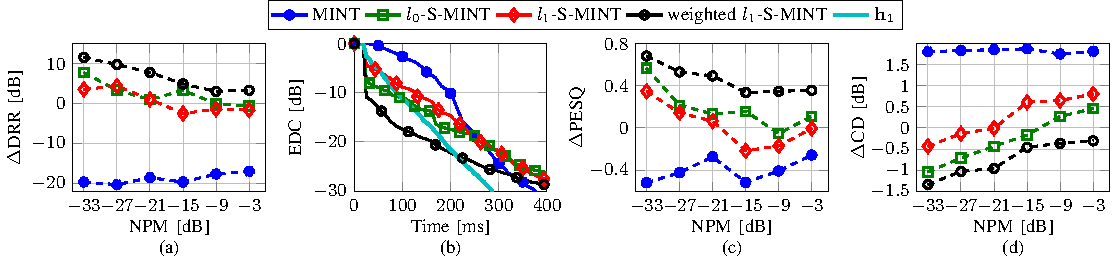
\includegraphics[scale=0.9]{Plots/perf_mint}
\caption{Performance of the MINT technique and sparsity-promoting MINT technique using different penalty functions for acoustic system $S_1$ in terms of (a) $\Delta$DRR, (b) EDC for an exemplary NPM of $-33$ dB, (c) $\Delta$PESQ, and (d) $\Delta$CD (intrusively selected weighting and penalty parameters $\eta$ and $\rho$).}
\label{fig: perf_mint}
\end{figure*}
\begin{figure*}[t!]
\centering
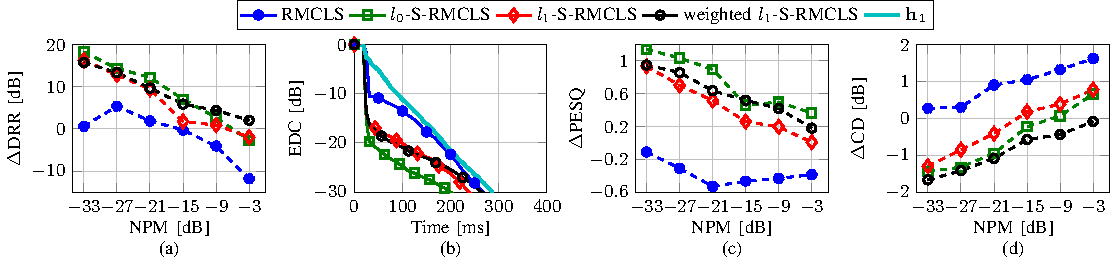
\includegraphics[scale=0.9]{Plots/perf_rmcls}
\caption{Performance of the RMCLS technique and sparsity-promoting RMCLS technique using different penalty functions for acoustic system $S_1$ in terms of (a) $\Delta$DRR, (b) EDC for an exemplary NPM of $-33$ dB, (c) $\Delta$PESQ, and (d) $\Delta$CD (intrusively selected weighting and penalty parameters $\eta$ and $\rho$).}
\label{fig: perf_rmcls}
\end{figure*}
\subsection{Sparsity-promoting acoustic multi-channel equalization techniques}
\label{sec: robust_increase}
In this section the performance of the considered least-squares equalization techniques, i.e., MINT, RMCLS, and PMINT, is investigated when incorporating the sparsity-promoting penalty functions presented in Section~\ref{sec: fsp}.
Although similar results are obtained for all considered acoustic systems, in this section only results for acoustic system $S_1$ are presented.
In order to illustrate the full potential of incorporating a sparsity-promoting penalty function, the weighting and penalty parameters $\eta$ and $\rho$ are selected from the set in~(\ref{eq: pars}) as the parameters minimizing the CD for each equalization technique, each penalty function, and each NPM (i.e., possibly different parameters are used for each equalization technique, each penalty function, and each NPM).
It should be noted that selecting the weighting and penalty parameters based on the CD is an intrusive procedure that cannot be applied in practice, since knowledge of the true RIRs is required in order to compute the reference signal and the resulting EIR.

\vskip 5pt
{\textit{Sparsity-promoting MINT}}
\vskip 5pt

Fig.~\ref{fig: perf_mint} depicts the performance of the MINT technique and sparsity-promoting MINT technique using different penalty functions in terms of $\Delta$DRR, EDC, $\Delta$PESQ, and $\Delta$CD. 
As expected, the $\Delta$DRR values presented in Fig.~\ref{fig: perf_mint}(a) show that MINT fails to suppress the reverberant energy, even worsening the DRR by approximately $20$ dB for all NPMs in comparison to $\mathbf{h}_1$. 
Furthermore, it can be observed that incorporating sparsity-promoting penalty functions significantly increases the robustness of MINT for all considered NPMs.
While incorporating the $l_0$- and $l_1$-norm penalty functions improves the DRR in comparison to $\mathbf{h}_1$ only for low NPMs, incorporating the weighted $l_1$-norm penalty function yields an improvement for all considered NPMs.
These results are confirmed in Fig.~\ref{fig: perf_mint}(b), which depicts the EDC of $\mathbf{h}_1$ and the EDCs of the EIRs obtained using MINT and the sparsity-promoting MINT techniques for an exemplary NPM of $-33$ dB.
It can be observed that the MINT technique completely fails to achieve dereverberation and even results in a slower reverberant energy decay rate than $\mathbf{h}_1$. 
Although the incorporation of the $l_0$- and $l_1$-norm penalty functions improves the reverberant energy decay rate in comparison to MINT, these penalty functions still yield a similar energy decay rate as $\mathbf{h}_1$.
On the other hand, incorporating the weighted $l_1$-norm penalty function is more advantageous and results in a faster reverberant energy decay rate than $\mathbf{h}_1$.
The larger reverberant energy suppression achieved by the weighted $l_1$-norm sparsity-promoting MINT technique is also reflected in the larger perceptual speech quality improvement illustrated by the $\Delta$PESQ and $\Delta$CD values in Figs.~\ref{fig: perf_mint}(c) and~\ref{fig: perf_mint}(d), where it can be observed that the weighted $l_1$-norm sparsity-promoting MINT technique is the only technique yielding an improvement in perceptual speech quality for all considered NPMs.

\vskip 5pt
{\textit{Sparsity-promoting RMCLS}}
\vskip 5pt
\begin{figure*}[t!]
\centering
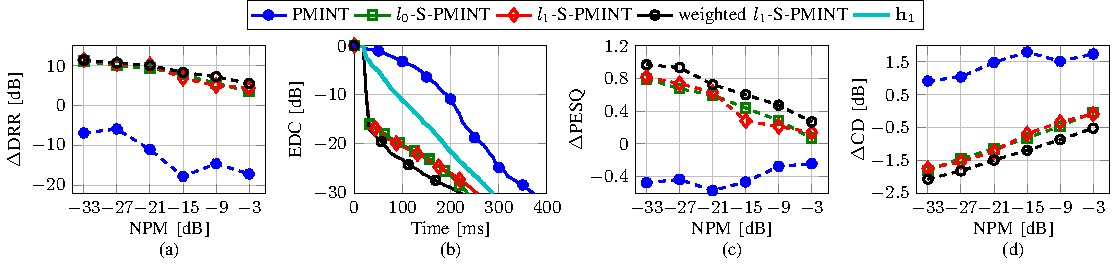
\includegraphics[scale=0.9]{Plots/perf_pmint}
\caption{Performance of the PMINT technique and sparsity-promoting PMINT technique using different penalty functions for acoustic system $S_1$ in terms of (a) $\Delta$DRR, (b) EDC for an exemplary NPM of $-33$ dB, (c) $\Delta$PESQ, and (d) $\Delta$CD (intrusively selected weighting and penalty parameters $\eta$ and $\rho$).}
\label{fig: perf_pmint}
\end{figure*}

Fig.~\ref{fig: perf_rmcls} depicts the performance of the RMCLS technique and sparsity-promoting RMCLS technique using different penalty functions in terms of $\Delta$DRR, EDC, $\Delta$PESQ, and $\Delta$CD. 
The $\Delta$DRR values presented in Fig.~\ref{fig: perf_rmcls}(a) show that for low NPMs the RMCLS technique slightly suppresses the reverberant energy, whereas for NPMs larger than $-15$~dB the RMCLS technique fails to achieve dereverberation and worsens the DRR in comparison to $\mathbf{h}_1$.
Furthermore, it can be observed that incorporating sparsity-promoting penalty functions in RMCLS significantly increases the reverberant energy suppression, with all penalty functions yielding a similar $\Delta$DRR for low NPMs.
As the NPM increases to $-3$ dB, the weighted $l_1$-norm sparsity-promoting RMCLS technique is the only technique achieving an (slight) improvement in DRR in comparison to $\mathbf{h}_1$. 
This increase in robustness when incorporating sparsity-promoting penalty functions is confirmed in Fig.~\ref{fig: perf_rmcls}(b), which depicts the EDC of $\mathbf{h}_1$ and the EDCs of the EIRs obtained using RMCLS and the sparsity-promoting RMCLS techniques for an exemplary NPM  of $-33$~dB.
It can be observed that while the RMCLS technique achieves a slightly faster reverberant energy decay rate than $\mathbf{h}_1$, the incorporation of all sparsity-promoting penalty functions results in a significantly faster energy decay rate.
In addition, it can be observed that for this exemplary NPM, the $l_0$-norm sparsity-promoting RMCLS technique yields the fastest reverberant energy decay rate, while the energy decay rate for the $l_1$- and weighted $l_1$-norm penalty functions is comparable.
The larger reverberant energy suppression achieved by the sparsity-promoting RMCLS techniques is also reflected in the larger perceptual speech quality improvement illustrated by the $\Delta$PESQ and $\Delta$CD values in Figs.~\ref{fig: perf_rmcls}(c) and~\ref{fig: perf_rmcls}(d), where it can be observed that the $l_0$-norm sparsity-promoting RMCLS technique typically yields the highest $\Delta$PESQ, whereas the weighted $l_1$-norm sparsity-promoting RMCLS technique always yields the lowest $\Delta$CD.
\begin{figure*}[t!]
  \centering
  % This file was created by matlab2tikz v0.4.0.
% Copyright (c) 2008--2013, Nico Schlömer <nico.schloemer@gmail.com>
% All rights reserved.
% 
% The latest updates can be retrieved from
%   http://www.mathworks.com/matlabcentral/fileexchange/22022-matlab2tikz
% where you can also make suggestions and rate matlab2tikz.
% 
% 
% 
\begin{tikzpicture}[font=\small]%
\begin{axis}[%
width=0.6\figurewidth,
height=1\figureheight,
axis on top,
scale only axis,
xmin=0,
xmax=3,
ymin=-7.8125,
xlabel style = {text width=1.55cm,align=center},
xlabel = {Time $t$ [s] \\ (a)},
xlabel style={yshift=0.5em},
ymax=4007.8125,
ylabel={Frequency $f$ [kHz]},
ylabel absolute, ylabel style={yshift=-1.4em},
ytick = {0,1000,2000,3000,4000},
yticklabels = {0,1,2,3,4},
colormap/jet,
%colorbar,
point meta min=-120,
point meta max=-40
]%
\addplot graphics [xmin=0.016,xmax=3.056,ymin=-7.8125,ymax=4007.8125] {Plots/spec_xd-1.png};%
\end{axis}%
\end{tikzpicture}%% This file was created by matlab2tikz v0.4.0.
% Copyright (c) 2008--2013, Nico Schlömer <nico.schloemer@gmail.com>
% All rights reserved.
% 
% The latest updates can be retrieved from
%   http://www.mathworks.com/matlabcentral/fileexchange/22022-matlab2tikz
% where you can also make suggestions and rate matlab2tikz.
% 
% 
%
\begin{tikzpicture}[font=\small]

\begin{axis}[%
width=0.6\figurewidth,
height=1\figureheight,
axis on top,
scale only axis,
xmin=0,
xmax=3,
ymin=-7.8125,
xlabel style = {text width=1.55cm,align=center},
xlabel = {Time $t$ [s] \\ (b)},
xlabel style={yshift=0.5em},
ymax=4007.8125,
%ylabel={Frequency $f$ [kHz]},
%ylabel absolute, ylabel style={yshift=-2.0em},
%ytick = {0,1000,2000,3000,4000},
yticklabels = {},
colormap/jet,
%colorbar,
point meta min=-120,
point meta max=-40
]
\addplot graphics [xmin=0.016,xmax=3.056,ymin=-7.8125,ymax=4007.8125] {Plots/spec_rev-1.png};
\end{axis}
\end{tikzpicture}%% This file was created by matlab2tikz v0.4.0.
% Copyright (c) 2008--2013, Nico Schlömer <nico.schloemer@gmail.com>
% All rights reserved.
% 
% The latest updates can be retrieved from
%   http://www.mathworks.com/matlabcentral/fileexchange/22022-matlab2tikz
% where you can also make suggestions and rate matlab2tikz.
% 
% 
%
\begin{tikzpicture}[font=\small]

\begin{axis}[%
width=0.6\figurewidth,
height=1\figureheight,
axis on top,
scale only axis,
xmin=0,
xmax=3,
ymin=-7.8125,
xlabel style = {text width=1.55cm,align=center},
xlabel = {Time $t$ [s] \\ (c)},
xlabel style={yshift=0.5em},
ymax=4007.8125,
%ylabel={Frequency [kHz]},
%ylabel absolute, ylabel style={yshift=-2.0em},
ytick = {0,1000,2000,3000,4000},
yticklabels = {},
colormap/jet,
colorbar,
colorbar style={
font = \footnotesize,
at={(1.05,0)},anchor=south west},
%colorbar,
point meta min=-120,
point meta max=-40
]
\addplot graphics [xmin=0.016,xmax=3.056,ymin=-7.8125,ymax=4007.8125] {Plots/spec_pmint-1.png};
\end{axis}
\end{tikzpicture}%
  % This file was created by matlab2tikz v0.4.0.
% Copyright (c) 2008--2013, Nico Schlömer <nico.schloemer@gmail.com>
% All rights reserved.
% 
% The latest updates can be retrieved from
%   http://www.mathworks.com/matlabcentral/fileexchange/22022-matlab2tikz
% where you can also make suggestions and rate matlab2tikz.
% 
% 
%
\begin{tikzpicture}[font=\small]%
\begin{axis}[%
width=0.6\figurewidth,
height=1\figureheight,
axis on top,
scale only axis,
xmin=0,
xmax=3,
ymin=-7.8125,
xlabel style = {text width=1.55cm,align=center},
xlabel = {Time $t$ [s] \\ (d)},%
xlabel style={yshift=0.5em},%
ymax=4007.8125,
ylabel={Frequency $f$ [kHz]},
ylabel absolute, ylabel style={yshift=-1.4em},
%ylabel={Frequency [kHz]},
%ylabel absolute, ylabel style={yshift=-2.0em},
ytick = {0,1000,2000,3000,4000},
yticklabels = {0,1,2,3,4},
colormap/jet,
%colorbar,
point meta min=-120,
point meta max=-40
]%
\addplot graphics [xmin=0.016,xmax=3.056,ymin=-7.8125,ymax=4007.8125] {Plots/spec_pmint_l0-1.png};%
\end{axis}%
\end{tikzpicture}%% This file was created by matlab2tikz v0.4.0.
% Copyright (c) 2008--2013, Nico Schlömer <nico.schloemer@gmail.com>
% All rights reserved.
% 
% The latest updates can be retrieved from
%   http://www.mathworks.com/matlabcentral/fileexchange/22022-matlab2tikz
% where you can also make suggestions and rate matlab2tikz.
% 
% 
%
\begin{tikzpicture}[font=\small]

\begin{axis}[%
width=0.6\figurewidth,
height=1\figureheight,
axis on top,
scale only axis,
xmin=0,
xmax=3,
ymin=-7.8125,
xlabel style = {text width=1.55cm,align=center},
xlabel = {Time $t$ [s] \\ (e)},
xlabel style={yshift=0.5em},
ymax=4007.8125,
%ylabel={Frequency [kHz]},
%ylabel absolute, ylabel style={yshift=-2.0em},
ytick = {0,1000,2000,3000,4000},
yticklabels = {},
colormap/jet,
%colorbar,
point meta min=-120,
point meta max=-40
]
\addplot graphics [xmin=0.016,xmax=3.056,ymin=-7.8125,ymax=4007.8125] {Plots/spec_pmint_l1-1.png};
\end{axis}
\end{tikzpicture}%% This file was created by matlab2tikz v0.4.0.
% Copyright (c) 2008--2013, Nico Schlömer <nico.schloemer@gmail.com>
% All rights reserved.
% 
% The latest updates can be retrieved from
%   http://www.mathworks.com/matlabcentral/fileexchange/22022-matlab2tikz
% where you can also make suggestions and rate matlab2tikz.
% 
% 
%
\begin{tikzpicture}[font=\small]%
\begin{axis}[%
width=0.6\figurewidth,
height=1\figureheight,
axis on top,
scale only axis,
xmin=0,
xmax=3,
ymin=-7.8125,
xlabel style = {text width=1.55cm,align=center},
xlabel = {Time $t$ [s] \\ (f)},
xlabel style={yshift=0.5em},
ymax=4007.8125,
%ylabel={Frequency [kHz]},
%ylabel absolute, ylabel style={yshift=-2.0em},
ytick = {0,1000,2000,3000,4000},
yticklabels = {},
colormap/jet,
colorbar,
colorbar style={
font = \footnotesize,
at={(1.05,0)},anchor=south west},
point meta min=-120,
point meta max=-40
]%
\addplot graphics [xmin=0.016,xmax=3.056,ymin=-7.8125,ymax=4007.8125] {Plots/spec_pmint_wl1-1.png};%
\end{axis}%
\end{tikzpicture}%
\caption{Spectrogram of (a) direct path and early reflections speech signal at the first microphone, (b) reverberant first microphone signal, (c) output signal obtained using PMINT, (d) output signal obtained using $l_0$-norm sparsity-promoting PMINT, (e) output signal obtained using $l_1$-norm sparsity-promoting PMINT, and (f) output signal obtained using weighted $l_1$-norm sparsity-promoting PMINT (acoustic system $S_1$, NPM $= -33$ dB, intrusively selected weighting and penalty parameters $\eta$ and $\rho$).}
\label{fig: spec}
\end{figure*}


\vskip 5pt
{\textit{Sparsity-promoting PMINT}}
\vskip 5pt
Fig.~\ref{fig: perf_pmint} depicts the performance of the PMINT technique and sparsity-promoting PMINT technique using different penalty functions in terms of $\Delta$DRR, EDC, $\Delta$PESQ, and $\Delta$CD. 
As expected, the $\Delta$DRR values presented in Fig.~\ref{fig: perf_pmint}(a) show that the PMINT technique fails to suppress the reverberant energy, even worsening the DRR in comparison to $\mathbf{h}_1$. 
Furthermore, it can be observed that incorporating sparsity-promoting penalty functions significantly increases the robustness of PMINT for all considered NPMs.
While all penalty functions result in a similarly large $\Delta$DRR for low NPMs, the weighted $l_1$-norm penalty function yields a slightly larger $\Delta$DRR than the $l_0$- and $l_1$-norm penalty functions for high NPMs.
These results are confirmed in Fig.~\ref{fig: perf_pmint}(b), which depicts the EDC of $\mathbf{h}_1$ and the EDCs of the EIRs obtained using PMINT and the sparsity-promoting PMINT techniques for an exemplary NPM of $-33$ dB.
It can be observed that the PMINT technique completely fails to achieve dereverberation and even results in a slower reverberant energy decay rate than $\mathbf{h}_1$.
The incorporation of all sparsity-promoting penalty functions results in a significantly faster reverberant energy decay rate, with the weighted $l_1$-norm penalty function yielding the fastest energy decay rate.
Furthermore, the $\Delta$PESQ and $\Delta$CD values depicted in Figs.~\ref{fig: perf_pmint}(c) and~\ref{fig: perf_pmint}(d) show that while PMINT worsens the perceptual speech quality in comparison to the reverberant signal $x_1(n)$, the incorporation of all sparsity-promoting penalty functions results in a significant improvement, with the weighted $l_1$-norm penalty function always yielding the highest $\Delta$PESQ and the lowest $\Delta$CD.

\vskip 2pt

\begin{table*}[t!]
\begin{center}
  \caption{Performance of the weighted $l_1$-norm sparsity-promoting MINT, RMCLS, and PMINT techniques (intrusively selected weighting and penalty parameters $\eta$ and $\rho$).}
  \label{tbl: wl1_s}
  \begin{tabularx}{\linewidth}{X|lrrr|rrrr|rrrr|}
    \toprule
    & \multicolumn{4}{c}{$\Delta$DRR [dB]} & \multicolumn{4}{|c|}{$\Delta$PESQ} & \multicolumn{4}{c|}{$\Delta$CD [dB]} \\
    \midrule
      & $S_1$ & $S_2$ & $S_3$ & Average &$S_1$ & $S_2$ & $S_3$ & Average& $S_1$ & $S_2$ & $S_3$ & Average\\
    \midrule
      weighted $l_1$-S-MINT & $6.7$ & $6.4$ & $2.8$ & $5.3$ & $0.5$ & $0.4$ & $0.0$ & $0.3$ & $-0.7$ & $-0.8$ & $0.1$ & $-0.5$\\
      weighted $l_1$-S-RMCLS & $8.5$ & $\bf 9.3$ & $\bf 8.3$ & $\bf8.7$ & $0.6$ & $0.6$ & $0.3$ & $0.5$ & $-0.9$ & $-1.1$ & $0.0$ & $-0.7$\\
      weighted $l_1$-S-PMINT & $\bf{8.8}$ & $8.7$ & $6.3$ & $7.9$ & $\bf 0.7$ & $\bf{0.8}$ & $\bf{0.6}$ &$\bf 0.7$ & $\bf -1.3$ & $\bf -1.6$ & $\bf{-0.8}$ & $\bf -1.2$\\
    \bottomrule
  \end{tabularx}
\end{center}
\end{table*}
In summary, these results show that incorporating sparsity-promoting penalty functions significantly increases the robustness of all considered equalization techniques against RIR perturbations. 
Furthermore, the weighted $l_1$-norm penalty function typically outperforms the $l_0$- and $l_1$-norm penalty functions in terms of the considered instrumental measures.

To further illustrate the advantage of promoting sparsity of the output signal in the STFT domain, Fig.~\ref{fig: spec} presents the spectrograms of the direct path and early reflections speech signal at the first microphone, the reverberant first microphone signal, the output signal obtained using the PMINT technique, and the output signals obtained using the sparsity-promoting PMINT techniques using different penalty functions for an exemplary NPM of $-33$ dB.
Comparing Figs.~\ref{fig: spec}(a) and~\ref{fig: spec}(b), it can be observed that due to the spectro-temporal smearing effect of reverberation, the spectrogram of the reverberant signal is significantly less sparse than the spectrogram of the direct path and early reflections speech signal.
Furthermore, Fig.~\ref{fig: spec}(c) shows that the non-robust PMINT technique introduces additional distortions, such that the resulting spectrogram is significantly less sparse than the spectrogram of the reverberant signal.
On the contrary, Fig.~\ref{fig: spec}(d) shows that incorporating the $l_0$-norm penalty function leads to a significantly more sparse spectrogram, largely suppressing the distortions introduced by the PMINT technique as well as partly suppressing the reverberant energy~(e.g., at $f \approx 1$ kHz).
In addition, Fig.~\ref{fig: spec}(e) shows that incorporating the $l_1$-norm penalty function results in a more sparse spectrogram than the $l_0$-norm penalty function, further suppressing the reverberant energy (e.g., at $t \approx 2.1$ s).
Finally, Fig.~\ref{fig: spec}(f) shows that an even more sparse spectrogram is obtained using the weighted $l_1$-norm penalty function, with the reverberant energy significantly suppressed (e.g., at $t \approx 0.5$ s and $t \approx 2.1$ s) and the spectro-temporal structure of the resulting signal closely resembling the spectro-temporal structure of the direct and early reflections speech signal in Fig.~\ref{fig: spec}(a).

\subsection{Comparison of the weighted $l_1$-norm sparsity-promoting acoustic multi-channel equalization techniques}
\label{sec: wl1}
Since it was shown in the previous section that incorporating the weighted $l_1$-norm penalty function typically yields the best performance, in this section the performance of the weighted $l_1$-norm sparsity-promoting MINT, RMCLS, and PMINT techniques is compared for all acoustic systems in Table~\ref{tbl: ac_sys} and all NPMs in~(\ref{eq: npm}).
The weighting and penalty parameters $\eta$ and $\rho$ are intrusively determined as in Section~\ref{sec: robust_increase}, i.e., as the parameters minimizing CD for each equalization technique, each acoustic system, and each NPM.
The performance of the different techniques is evaluated in terms of $\Delta$DRR, $\Delta$PESQ, and $\Delta$CD, and the presented performance measures are averaged over all considered NPMs. 

Table~\ref{tbl: wl1_s} presents the obtained $\Delta$DRR, $\Delta$PESQ, and $\Delta$CD values for all considered acoustic systems and techniques.
In addition, the average performance measures over all acoustic systems are also presented.
First, it can be observed that the weighted $l_1$-norm sparsity-promoting MINT technique results in the lowest performance in terms of all performance measures.
Since the MINT technique is very sensitive to RIR perturbations (cf. Fig.~\ref{fig: perf_mint}), the robustness increase that can be obtained by incorporating signal-dependent penalty functions is also limited.
Second, it can be observed that the weighted $l_1$-norm sparsity-promoting PMINT and RMCLS techniques yield a high reverberant energy suppression in terms of $\Delta$DRR, with the weighted $l_1$-norm sparsity-promoting PMINT technique resulting in a similar $\Delta$DRR (for $S_1$ and $S_2$) or slightly lower $\Delta$DRR (for $S_3$) than the weighted $l_1$-norm sparsity-promoting RMCLS technique.
Finally, it can be observed that for all considered acoustic systems, the weighted $l_1$-norm sparsity-promoting PMINT technique yields the largest perceptual speech quality improvement, outperforming the weighted $l_1$-norm sparsity-promoting RMCLS technique in terms of $\Delta$PESQ and $\Delta$CD.
While the weighted $l_1$-norm sparsity-promoting PMINT technique always improves the perceptual speech quality in comparison to the reverberant signal as indicated by positive $\Delta$PESQ and negative $\Delta$CD values, the weighted $l_1$-norm sparsity-promoting RMCLS technique might fail to yield an improvement, as indicated by $\Delta$CD $= 0.0$ dB for acoustic system $S_3$.
The advantage of building upon the PMINT technique lies in its control of the early reflections in the EIR, hence better preserving the perceptual speech quality of the output signal. 

Summarizing these simulation results, we conclude that the weighted $l_1$-norm sparsity-promoting PMINT technique is a robust and perceptually advantageous equalization technique, yielding a high reverberant energy suppression and outperforming all other considered techniques in terms of the perceptual speech quality improvement.

\begin{table*}[t!]
\begin{center}
  \caption{Performance of the weighted $l_1$-norm sparsity-promoting PMINT technique ($\eta = 10^{-7}$, $\rho = 10^{-4}$) and regularized PMINT technique ($\delta = 10^{-6}$).}
  \label{tbl: spa_reg1}
  \begin{tabularx}{\linewidth}{X|lrrr|rrrr|rrrr|}
    \toprule
    & \multicolumn{4}{c|}{$\Delta$DRR [dB]} & \multicolumn{4}{c|}{$\Delta$PESQ} & \multicolumn{4}{c|}{$\Delta$CD [dB]} \\
    \midrule
      & $S_1$ & $S_2$ & $S_3$ & Average& $S_1$ & $S_2$ & $S_3$ & Average &  $S_1$ & $S_2$ & $S_3$ & Average\\
    \midrule
      Weighted $l_1$-S-PMINT & $\bf{8.2}$ & $\bf{7.0}$ & $\bf{6.4}$ &$\bf 7.2$ & $\bf{0.6}$ & $0.5$ & $\bf{0.6}$ & $\bf 0.6$ & $\bf{-1.2}$ & $-1.2$ & $-0.7$ & $-1.0$\\
      Regularized PMINT & $7.9$ & $\bf{7.0}$ & $5.4$ & $6.8$ & ${0.5}$ & $\bf{0.6}$ & ${0.5}$ & $0.5$ & $-1.1$ & $\bf{-1.3}$ & $\bf{-0.8}$ & $\bf -1.1$\\
    \bottomrule
  \end{tabularx}
\end{center}
\end{table*}
\begin{table*}[t!]
\begin{center}
  \caption{Performance of the weighted $l_1$-norm sparsity-promoting PMINT technique ($\eta = 10^{-7}$, $\rho = 10^{-3}$) and regularized PMINT technique ($\delta = 10^{-1}$).}
  \label{tbl: spa_reg2}
  \begin{tabularx}{\linewidth}{X|lrrr|rrrr|rrrr|}
    \toprule
    & \multicolumn{4}{c|}{$\Delta$DRR [dB]} & \multicolumn{4}{c|}{$\Delta$PESQ} & \multicolumn{4}{c|}{$\Delta$CD [dB]} \\
    \midrule
      & $S_1$ & $S_2$ & $S_3$ & Average& $S_1$ & $S_2$ & $S_3$ & Average &  $S_1$ & $S_2$ & $S_3$ & Average\\
    \midrule
      weighted $l_1$-S-PMINT & $\bf{8.8}$ & $\bf{7.4}$ & $\bf{6.6}$ & $\bf 7.6$  & $\bf{0.7}$ & $\bf{0.6}$ & $\bf{0.7}$ & $\bf{0.7}$ & $\bf{-1.3}$ & $\bf{-1.3}$ & $\bf{-0.6}$ & $\bf -1.1$\\
      regularized PMINT & $3.4$ & $5.8$ & $3.6$ & $4.3$ & $0.2$ & $0.5$ & $0.2$ & $0.3$ & $-0.6$ & $-0.8$ & $-0.3$ & $-0.6$\\
    \bottomrule
  \end{tabularx}
\end{center}
\end{table*}


\subsection{Performance of the weighted $l_1$-norm sparsity-promoting PMINT technique for different weighting and penalty parameters}
\label{sec: eta_rho}

In order to gain more insight on the weighted $l_1$-norm sparsity-promoting PMINT technique, in this section we analyze its performance for different choices of the weighting and penalty parameters $\eta$ and $\rho$.
Fig.~\ref{fig: eta_rho} depicts the $\Delta$CD values obtained using the weighted $l_1$-norm sparsity-promoting PMINT technique with different values of $\eta$ and $\rho$ for the exemplary acoustic system $S_1$ and an NPM of $-33$ dB.
It should be noted that similar results are obtained for all considered performance measures, acoustic systems, and NPMs.
It can be observed that for a fixed weighting parameter $\eta$ (e.g., $\eta = 10^{-5}$) changing the penalty parameter $\rho$ can yield a significant change in the obtained $\Delta$CD (e.g., up to $3$~dB).
For a fixed penalty parameter $\rho$ (e.g., $\rho = 10^{-3}$) changing the weighting parameter $\eta$ can also yield a significant change in the obtained $\Delta$CD (e.g., up to $3$~dB).
\begin{figure}[b!]
  \centering
  % This file was created by matlab2tikz.
%
%The latest updates can be retrieved from
%  http://www.mathworks.com/matlabcentral/fileexchange/22022-matlab2tikz-matlab2tikz
%where you can also make suggestions and rate matlab2tikz.
%
\begin{tikzpicture}

\begin{axis}[%
width=0.838\figurewidth,
height=\figureheight,
at={(0\figurewidth,0\figureheight)},
scale only axis,
point meta min=-2.07297295874699,
point meta max=2.52425577852429,
axis on top,
xmin=0.5,
xmax=7.5,
xlabel={$\rho$},
y dir=reverse,
ymin=0.5,
ymax=7.5,
ylabel={$\eta$},
axis background/.style={fill=white},
colormap/jet,
colorbar
]
\addplot [forget plot] graphics [xmin=0.5, xmax=7.5, ymin=0.5, ymax=7.5] {eta_rho_depend-1.png};
\end{axis}
\end{tikzpicture}%
\caption{Performance of the weighted $l_1$-norm sparsity-promoting PMINT technique in terms of $\Delta$CD for several weighting and penalty parameters $\eta$ and $\rho$ (acoustic system $S_1$, NPM $= -33$ dB).}
\label{fig: eta_rho}
\end{figure}
Hence unfortunately, the performance of the weighted $l_1$-norm sparsity-promoting PMINT technique is rather dependent on the choice of the weighting and penalty parameters. 
However, as it will be shown in Section~\ref{sec: reg_spa}, once a set of optimal weighting and penalty parameters has been determined, the same parameters can be used for different acoustic systems and NPMs to obtain a near-to-optimal performance.


\subsection{Comparison of the weighted $l_1$-norm sparsity-promoting PMINT and regularized PMINT techniques}
\label{sec: reg_spa}
In this section, we compare the performance between incorporating the proposed signal-dependent weighted $l_1$-norm penalty function and the signal-independent regularization term in the PMINT technique for all acoustic systems in Table~\ref{tbl: ac_sys} and NPMs in~(\ref{eq: npm}).
In contrast to Sections~\ref{sec: robust_increase} and~\ref{sec: wl1}, for a more realistic evaluation the same weighting and penalty parameters $\eta$ and $\rho$ are now used in the weighted $l_1$-norm sparsity-promoting PMINT technique for all acoustic systems and NPMs.
Similarly, the same regularization parameter $\delta$ is used in the regularized PMINT technique for all acoustic systems and NPMs.
To systematically compare both techniques, we investigate the performance for two different settings of these parameters, i.e., the parameters $\eta$, $\rho$, and $\delta$ are determined as the parameters minimizing CD for acoustic system $S_1$ and
\begin{itemize}
\item[i)] NPM $ = -33$ dB, resulting in $\eta = 10^{-7}$, $\rho = 10^{-4}$, and $\delta = 10^{-6}$, and
\item[ii)] NPM $ = -3$ dB, resulting in $\eta = 10^{-7}$, $\rho = 10^{-3}$, and $\delta = 10^{-1}$.
\end{itemize}
As indicated by the obtained parameter values, the weighting and penalty parameters yielding a high performance for the sparsity-promoting PMINT technique do not change significantly for different NPMs, whereas the regularization parameter yielding a high performance for the regularized PMINT technique significantly changes for different NPMs.
This is not surprising since the regularized cost function in~(\ref{eq: rls_cost}) explicitly incorporates an RIR perturbation model in the filter design where the appropriate regularization parameter depends on the distortion energy due to RIR perturbations, whereas the sparsity-promoting cost function in~(\ref{eq: cost_sp2}) only relies on characteristics of clean speech signals.
The performance of both techniques is evaluated in terms of $\Delta$DRR, $\Delta$PESQ, and $\Delta$CD, and the presented performance measures are averaged over all considered NPMs. 

Table~\ref{tbl: spa_reg1} presents the obtained $\Delta$DRR, $\Delta$PESQ, and $\Delta$CD values for both considered techniques using the parameters in case i).
In addition, the average performance measures over all acoustic systems are also presented.
It can be observed that for these parameters the sparsity-promoting PMINT technique and the regularized PMINT technique yield a very similar performance in terms of all performance measures.
While the sparsity-promoting PMINT technique results in a slightly higher $\Delta$DRR and $\Delta$PESQ, the regularized PMINT technique results in a slightly lower $\Delta$CD.

Table~\ref{tbl: spa_reg2} presents the obtained $\Delta$DRR, $\Delta$PESQ, and $\Delta$CD values for both considered techniques using the parameters in case ii).
In addition, the average performance measures over all acoustic systems are also presented.
It can now be observed that for these parameters the sparsity-promoting PMINT technique significantly outperforms the regularized PMINT technique in terms of all performance measures, yielding on average a higher $\Delta$DRR of $3.3$~dB, a higher $\Delta$PESQ of $0.4$, and a lower $\Delta$CD of $0.5$ dB.

In summary, these results show that the proposed signal-dependent sparsity-promoting PMINT technique yields a similar or significantly better dereverberation performance than the signal-independent regularized PMINT technique, depending on the used weighting, penalty, and regularization parameters.
This shows the potential of incorporating sparsity-promoting penalty functions which exploit well-established characteristics of clean speech signals to increase the robustness of equalization techniques against RIR perturbations.
Combining signal-independent regularization based on an RIR perturbation model and signal-dependent penalty functions remains a topic for future investigation.
% Furthermore, it has been shown that while the regularization parameter that yields a high performance in the regularized PMINT technique highly depends on the NPM, the weighting and penalty parameters that yield a high performance in the sparsity-promoting PMINT technique do not significantly change with changing NPM levels.
% It should be noted that the proposed sparsity-promoting PMINT technique significantly increases the robustness against RIR perturbations exploiting only well established characteristics of clean speech signals, which can be considered to be a very good result.
% Incorporating signal-dependent penalty functions in more robust signal-independent equalization techniques to further increase the robustness against RIR perturbations remains a topic for future investigation.

\section{Conclusion}
In this paper we have proposed to increase the robustness of acoustic multi-channel equalization techniques against RIR perturbations using signal-dependent penalty functions, such that the output signal better resembles a clean speech signal.
We have proposed to extend the cost function of least-squares equalization techniques with different sparsity-promoting penalty functions, i.e., the $l_0$-norm, the $l_1$-norm, and the weighted $l_1$-norm.
The sparsity-promoting filters have been iteratively computed based on the ADMM.
Simulation results show that incorporating sparsity-promoting penalty functions in all considered equalization techniques, i.e., MINT, RMCLS, and PMINT, significantly increases the robustness against RIR perturbations and suppresses artifacts generated by non-robust equalization techniques.
In addition, it is shown that the weighted $l_1$-norm penalty function typically outperforms the $l_0$- and $l_1$-norm penalty functions, with the weighted $l_1$-norm sparsity-promoting PMINT technique yielding a high reverberant energy suppression and outperforming all other considered techniques in terms of perceptual speech quality improvement.
Finally, it is shown that the proposed signal-dependent weighted $l_1$-norm sparsity-promoting PMINT technique yields a similar or significantly better dereverberation performance than the signal-independent regularized PMINT technique, confirming the advantage of using signal-dependent penalty functions for robust dereverberation filter design and motivating future research in this direction.


\bibliographystyle{IEEEtran}
\bibliography{refs}

\begin{IEEEbiography}[{
\includegraphics[width=1in,height=1.25in,clip,keepaspectratio]{Plots/ina1}}]
  {Ina Kodrasi} received the Master of Science degree in Communications, Systems and Electronics in 2010 from Jacobs University Bremen, Germany and the PhD degree in 2015 from the University of Oldenburg, Germany.
  From 2010 to 2015 she worked as an early stage researcher at the Signal Processing Group of the University of Oldenburg.
  From 2010 to 2011 she was also with the Fraunhofer Institute for Digital Media Technology (IDMT), Project group Hearing, Speech and Audio Technology in Oldenburg where she worked on microphone array beamforming.
  Since December 2015 she is a postdoctoral researcher at the Signal Processing Group of the University of Oldenburg in the field of speech dereverberation and noise reduction.

\end{IEEEbiography}

\begin{IEEEbiography}[{
\includegraphics[width=1in,height=1.25in,clip,keepaspectratio]{Plots/doclo_2013_1}}]{Simon Doclo}
  (S'95, M'03) Simon Doclo received the M.Sc. degree in electrical engineering and the Ph.D. degree in applied sciences from the Katholieke Universiteit Leuven, Belgium, in 1997 and 2003. From 2003 to 2007 he was a Postdoctoral Fellow with the Research Foundation – Flanders at the Electrical Engineering Department (Katholieke Universiteit Leuven) and the Adaptive Systems Laboratory (McMaster University, Canada). From 2007 to 2009 he was a Principal Scientist with NXP Semiconductors at the Sound and Acoustics Group in Leuven, Belgium. Since 2009 he is a full professor at the University of Oldenburg, Germany, and scientific advisor for the project group Hearing, Speech and Audio Technology of the Fraunhofer Institute for Digital Media Technology. His research activities center around signal processing for acoustical and biomedical applications, more specifically microphone array processing, active noise control, acoustic sensor networks and hearing aid processing.
Prof. Doclo received the Master Thesis Award of the Royal Flemish Society of Engineers in 1997 (with Erik De Clippel), the Best Student Paper Award at the International Workshop on Acoustic Echo and Noise Control in 2001, the EURASIP Signal Processing Best Paper Award in 2003 (with Marc Moonen) and the IEEE Signal Processing Society 2008 Best Paper Award (with Jingdong Chen, Jacob Benesty, Arden Huang). He was member of the IEEE Signal Processing Society Technical Committee on Audio and Acoustic Signal Processing (2008-2013) and Technical Program Chair for the IEEE Workshop on Applications of Signal Processing to Audio and Acoustics (WASPAA) in 2013. Prof. Doclo has served as guest editor for several special issues (IEEE Signal Processing Magazine, Elsevier Signal Processing) and is associate editor for IEEE/ACM Transactions on Audio, Speech and Language Processing and EURASIP Journal on Advances in Signal Processing. 
\end{IEEEbiography}

\end{document}


\grid
